\documentclass{article}
\usepackage{listings}


\usepackage{amsmath,amsfonts,amsthm,amssymb,amsopn,bm}
% \usepackage{fullpage}
\usepackage[margin=.9in]{geometry}
\usepackage{graphicx}
% \usepackage{fullpage}
% \usepackage[paper=letterpaper,margin=1in,includeheadfoot,footskip=0.25in,headsep=0.25in]{geometry}
\usepackage{url}
\usepackage[usenames,dvipsnames]{color}
% \usepackage[pdfborder={0 0 1},colorlinks=true,citecolor=black,plainpages=false]{hyperref}
\usepackage{fancyhdr}
\usepackage[ruled]{algorithm2e}
% \usepackage{multirow}
\newcommand{\field}[1]{\mathbb{#1}}
\newcommand{\1}{\mathbf{1}}
\newcommand{\E}{\mathbb{E}} % real domain
\renewcommand{\P}{\mathbb{P}} % real domain
\newcommand{\R}{\field{R}} % real domain
% \newcommand{\C}{\field{C}} % complex domain
\newcommand{\F}{\field{F}} % functional domain

\newcommand{\T}{^{\textrm T}} % transpose


\def\diag{\text{diag}}

%% operator in linear algebra, functional analysis
\newcommand{\inner}[2]{#1\cdot #2}
\newcommand{\norm}[1]{\left\|#1\right\|}
\newcommand{\twonorm}[1]{\|#1\|_2^2}
% operator in functios, maps such as M: domain1 --> domain 2
\newcommand{\Map}[1]{\mathcal{#1}}
\renewcommand{\theenumi}{\alph{enumi}} 

\newcommand{\Perp}{\perp \! \! \! \perp}

\newcommand\independent{\protect\mathpalette{\protect\independenT}{\perp}}
\def\independenT#1#2{\mathrel{\rlap{$#1#2$}\mkern2mu{#1#2}}}
\newcommand{\vct}[1]{\boldsymbol{#1}} % vector
\newcommand{\mat}[1]{\boldsymbol{#1}} % matrix
\newcommand{\cst}[1]{\mathsf{#1}} % constant
\newcommand{\ProbOpr}[1]{\mathbb{#1}}
\newcommand{\grade}[1]{\small\textcolor{magenta}{\emph{[#1 points]}} \normalsize}
\date{{}}

\setlength\parindent{0px}

\begin{document}
\title{Homework \#2}
\author{\normalsize{CSE 546: Machine Learning}\\
\normalsize{Mitchell Vollger} \\
\normalsize{Collaborators: April Lo, David Read, Anna Minkina} \\
\normalsize{Due: 11/1/2018  11:59 PM}}
\maketitle

\section{A Taste of Learning Theory}
1. \grade{2}
Let $X$ be a random feature vector in $\R^d$ and $Y$ be a random label in $\{1,\dots,K\}$ for some $K \in \mathbb{N}$ drawn from a joint distribution $P_{XY}$. 
A \emph{randomized classifier} $\delta(x)$ takes an $x\in \R^d$ as input and outputs an element $y \in \{1,\dots,K\}$ with probability $\alpha(x,y) := P(\delta(x) = y)$, where $\sum_{y=1}^K \alpha(x,y) = 1$ for all $x$.
For any classifier $\delta$ we define the \emph{risk} as
\begin{align*}
R(\delta) := \E_{XY,\delta}[ \1\{ \delta(X) \neq Y \}]
 % = \E_X[ \E_{Y|X}[ \1\{\delta(x) \neq Y \} | X=x ] ]
\end{align*}
where $\1(\mathcal{E})$ is the indicator function for the event $\mathcal{E}$ (the
function takes the value $1$ if $\mathcal{E}$ occurs and $0$ otherwise).
We say a classifier $\delta$ is \emph{deterministic} if $\alpha(x,y) \in \{0,1\}$ for all $x,y$.
A Bayes classifier is defined as $\delta_* \in \arg\inf_\delta R(\delta)$ where the infimum is taken over all randomized classifiers (note it may not be unique). 
For an arbitrary $P_{XY}$, characterize the set of all Bayes Classifiers (i.e., for a given $x$ what are permissible Bayes classifiers in terms of $\alpha(x,y)$).
Then propose a deterministic decision rule that is a Bayes classifier.\\



\section*{Problem 1 answer }




\section*{}
2. \grade{8} 
For $i=1,\dots,n$ let $(x_i,y_i) \overset{i.i.d.}{\sim} P_{XY}$ where $y_i \in \{-1,1\}$ and $x_i$ lives in some set $\mathcal{X}$ ($x_i$ is not necessarily a vector). 
The $0/1$ loss, or \emph{risk}, for a deterministic classifier $f:\mathcal{X} \rightarrow \{ -1,1 \}$ is defined as:
\begin{align*}
R(f) = \mathbb E_{XY} [\1(f(X)\neq Y)]
\end{align*}
where $\1(\mathcal{E})$ is the indicator function for the event $\mathcal{E}$ (the
function takes the value $1$ if $\mathcal{E}$ occurs and $0$ otherwise).
The expectation is with respect to the underlying distribution $P_{XY}$ on $(X,Y)$.
Unfortunately, we don't know $P_{XY}$ exactly, but we do have our i.i.d. samples $\{(x_i,y_i)\}_{i=1}^n$ drawn from it.
Define the \emph{empirical risk} as 
\begin{align*}
\widehat R_n(f) = \frac{1}{n} \sum_{i=1}^n \mathbf{1}(f(x_i)\neq y_i) 
\end{align*}
which is just an empirical estimate of our loss.
Recall Hoeffding's inequality: if $Z_1,\dots,Z_m$ are i.i.d. random variables on the interval $[a,b]$ where $\E[Z_i] = \mu$ and $\widehat{\mu} = \frac{1}{m} \sum_{i=1}^m Z_i$, then 
\begin{align*}
\P\left( |\mu - \widehat{\mu}| \geq \epsilon \right) \leq 2 \exp\left(- \frac{2 m \epsilon^2}{(b-a)^2}\right).
\end{align*}

\begin{enumerate}
  \item Suppose a domain expert who has not seen your freshly drawn data $\{(x_i,y_i)\}_{i=1}^n$ gives you a classifying rule $\widetilde{f}:\mathcal{X} \rightarrow \{-1,1\}$. We wish to estimate the true risk $R(\widetilde{f})$ of this classifying rule using the empirical risk $\widehat{R}_n(\widetilde{f})$. Justify the use of Hoeffding's inequality, and use it to find a value of $A$ such that
  \begin{align*}
  \P( | \widehat{R}_n(\widetilde{f}) - R(\widetilde{f}) | \leq A ) \geq 1- \delta.
  \end{align*}
  \item After seeing the confidence interval, the domain expert is not satisfied with her classifying rule $\widetilde{f}$. Because she understands the underlying process that generated the data, she proposes a finite set of alternative classifying rules $\mathcal{F} = \{ f_1,\dots,f_k \}$ that may fit the data better.
  The ``best in class'' function $f^*$ is:
  \[
  f^* = \arg\min_{f \in \mathcal{F}} R(f) \, . 
  \]
  Note that $R(f^*)$ is the best true loss we could hope to achieve using functions in $\mathcal{F}$.
  If we replace $\widetilde{f}$ with $f^*$ in part a., does the same confidence interval hold? Why or why not?
  \item Of course, determining $f^*$ would require exact knowledge of $R(f)$, which requires exact knowledge of $P_{XY}$, which we don't have. 
  As an alternative, you propose to use the \emph{empirical risk minimizer} (ERM):
  \begin{align*}
  \widehat f = \arg\min_{f\in\mathcal{F}} \widehat R_n(f).
  \end{align*}
  If we replace $\widetilde{f}$ with $\widehat{f}$ in part a., does the same confidence interval hold? Why or why not? 
  \item Come up with a \textbf{simple} example (i.e., give a $P_{XY},\mathcal{F}$) where for any number of observations $n$ we have $\widehat{R}_n(\widehat{f})=0$ and $R(\widehat{f})=1/2$ where $\widehat{f} = \arg\min_{f \in \mathcal{F}} \widehat{R}_n(f)$.  
  \item  Provide a confidence interval that simultaneously holds for the losses of all $f \in \mathcal{F}$, with probability of error $\delta$. In other words, provide a value $B$ so that:
\[
\P( \textrm{for all } f\in\mathcal{F}, \, |\widehat R_n(f) -  R(f)|
\leq B ) \geq 1- \delta
\]
Show your steps. (Hint: for events $\mathcal{E}_1, \mathcal{E}_2, \ldots, \mathcal{E}_k$, the ``union bound'' states that  $\P(\mathcal{E}_1 \textrm{ or } \mathcal{E}_2 \textrm{ or } \dots \text{ or } \mathcal{E}_k) = \P(\bigcup_{i=1}^k \mathcal{E}_i ) \leq \sum_{i=1}^k \P(\mathcal{E}_k)$.)
\item Noting that $\widehat{f} \in \mathcal{F}$, provide a confidence interval for the loss of $\widehat f$ that holds with
  probability greater than $1-\delta$. In other words, we are seeking
  a bound on $|R(\widehat f)-\widehat R_n(\widehat f)|$ that holds with probability greater than $1-\delta$.

\item Provide a bound on how close your loss, using the ERM, is
  to the best possible loss (in the hypothesis space). 
  Specifically, provide a value $C$ so that the following holds with probability greater than $1-\delta$,
  \[
  R(\widehat f) - R(f^*) \leq C
  \]
  The quantity $R(\widehat f) - R(f^*)$ is often referred to as the \emph{excess risk}.

\item Fix an $f \in \mathcal{F}$ and suppose $R(f) > \epsilon$. 
Show that $\P( \widehat{R}_n(f) = 0 ) \leq (1-\epsilon)^n \leq e^{-n \epsilon}$.
Leverage this insight to show that with probability at least $1-\delta$ 
\begin{align*}
\widehat{R}_n(\widehat{f})=0 \quad \implies \quad  R(\widehat f) - R(f^*) \leq \frac{\log(|\mathcal{F}|/\delta)}{n}
\end{align*}
where $\widehat f = \arg\min_{f\in\mathcal{F}} \widehat R_n(f)$. 

\item \label{last_part} Let us understand how large a hypothesis class we can utilize,
  i.e. how large $|\mathcal{F}|$ can be? Suppose we know we will be provided with a training set of
  size $n$, and, before we look at our training data, we choose the
  a hypothesis class $\mathcal{F}$ as a function of the sample size $n$. As we get
  more data, we would expect that we can utilize a larger hypothesis
  class. Let us examine this more quantitatively. We can think of
  learning being possible if our regret tends to $0$ as $n$ becomes
  large (with a probability of error less than  $\delta$). Let us determine if learning is possible in each of the
  following cases. For the following cases, does the above suggest that we are able to learn, and if so, what is our excess risk as a function of $n$ in big-O notation?
\begin{enumerate}
\item $|\mathcal{F}|$ is a constant.\\
\item $|\mathcal{F}|=n^p$ for some constant $p$.\\
\item $|\mathcal{F}|=\exp(\sqrt{n})$.\\
\item $|\mathcal{F}|=\exp(10 n)$. \\
\end{enumerate}
\end{enumerate}
Your answers to part \ref{last_part} are one interpretation as to when and why learning
complex models is possible (from a statistical perspective). 
Of particular interest is when $\mathcal{F}$ is allowed to be infinite in which more advanced tools are necessary. 
To provide intuition we note that $n$ points in $d$-dimensions can be labeled by a hyperplane $w$ in at most $O(n^d)$ ways (i.e., $|\{ \text{sign}(\mathrm{X} w) : w \in \R^d \}| = O(n^d)$ for fixed $\mathrm{X} \in \R^{n \times d}$).
While more advanced tools (e.g., VC dimension, covering numbers, etc.) are necessary to formally prove the learning rates for infinite classes, thinking about this number of sign patterns and how this relates to $|\mathcal{F}|$ is instructive.



\section*{Problem 2a Answer}
Given that the data is iid and a Bernoulli random variable we can use the Hoeffding's inequality, as long as $\Tilde{f}$ does not make the data points not iid. 

\begin{align*}
    P(|\Hat{R}_n(\Tilde{f}) - R_n(\Tilde{f}) | \leq A ) & \geq 1- \delta  \\
    -P(|\Hat{R}_n(\Tilde{f}) - R_n(\Tilde{f}) |\leq A ) & \leq  \delta - 1  \\
    1-P(|\Hat{R}_n(\Tilde{f}) - R_n(\Tilde{f}) | \leq A) & \leq  \delta \\
    P(|\Hat{R}_n(\Tilde{f}) - R_n(\Tilde{f}) | \geq A) & \leq  \delta \\
\end{align*}
This now looks like Hoeffding's inequality with A instead of $\epsilon$. Therefore we can solve for A in the following equation. 
\begin{align*}
    \delta & = 2 * exp(\frac{-2 n A^2}{ 1 - 0})\\
    \log( \delta / 2 )  & = \frac{-2 n A^2}{ 1})\\
    A^2 & = \frac{1}{ -2n} \log( \delta / 2 ) \\
    A & = \sqrt{ \frac{1}{2n}) \log( 2/\delta) } \\
\end{align*}


\section*{Problem 2b Answer}
The inequality holds for any iid Bernoulli random variables and a function that keeps those samples iid. Because $f*$ has not been biased/estimated from that data the same confidence interval must hold, and the same value for A. If $f*$ had been chosen/optimized using the data, this would not be the case. 

\section*{Problem 2c Answer}
The same confidence interval does not hold because the use of the inequality is not valid in this case. It is not valid because $\Hat{f}$ was created/chosen by using the data. This makes the data biased with $\Hat{f}$ so they are no longer iid. 


\section*{Problem 2d Answer}
Let us pretend that $X$ is totally uninformative of $y$ and that $y$ is just a coin flip with that is $\{-1,1\}$ with equal probability for both outcomes.

Next let the size of $F$ be one, with the one function being k-nearest neighbors with k equal to one. In other words, just define a function such that each set of $X$ coordinates will map to its $y$ label. This perfectly predicts the training data, but will just reflect the randomness of y for new data. \\

Thus the risk on the data will be zero. 
$$\Hat{R}(\Hat{f})_n = \frac{1}{n} \sum_{i=1}^n 1(\hat{f}(x_i) \ne y_i ) = 0$$
However, new data points will be classified without any information (because $X$ is not informative) so they will be correct half the time. 
$$R(\Hat{f}) = E_{xy}[1(\Hat{f}(x) \ne y)] = 1/2 $$

By definition $\hat{f}$ is the argmin of $F$ because it is the only function in $F$. 


\section*{Problem 2e Answer}

\section*{Problem 2f Answer}
It can be bounded by $B$ because in part e it was proven that for any and all $f$ in $F$ we could use the bound $B$. Thus $f$ must also be bounded by $B$. 

\section*{Problem 2g Answer}

\begin{align*}
    R(\hat{f}) - R(f^*) & \leq C \\
    R(\hat{f}) - R(f^*) & =   R(\hat{f}) - \Hat{R}_n(\Hat{f}) + \Hat{R}_n(\Hat{f})  - (R(f^*) -\Hat{R}_n(f^*) + \Hat{R}_n(f^*) ) \\
\end{align*}
However $\Hat{R}_n(\Hat{f}) - \Hat{R}_n(f^*) ) \leq 0 $, so:\\
\begin{align*}
    R(\hat{f}) - \Hat{R}_n(\Hat{f}) + \Hat{R}_n(\Hat{f})  - (R(f^*) -\Hat{R}_n(f^*) + \Hat{R}_n(f^*) ) & \leq 
    R(\hat{f}) - \Hat{R}_n(\Hat{f})  - (R(f^*) -\Hat{R}_n(f^*)) \\
    R(\hat{f}) - \Hat{R}_n(\Hat{f})  - (R(f^*) -\Hat{R}_n(f^*)) & \leq |R(\hat{f}) - \Hat{R}_n(\Hat{f})|  + |R(f^*) -\Hat{R}_n(f^*)| \\
\end{align*}
But we have shown that for any $f$ both of these terms, $|R(\hat{f}) - \Hat{R}_n(\Hat{f})|$  and $|R(f^*) -\Hat{R}_n(f^*)|$, are bound by $B$ thus together they must be bounded by $2B$. Therefore we can say that we can bound  $R(\hat{f}) - R(f^*) & \leq C$ with $C=2B$.

\section*{Problem 2h Answer}

\section*{Problem 2i Answer}

























\section{Programming: Lasso}

Given $\lambda >0$ and data $(x_1,y_1),\dots,(x_n,y_n)$, the Lasso is the problem of solving
\begin{equation}\label{eq:lasso}
  \arg\min_{{w}\in \R^d, b \in \R} \sum_{i=1}^n { (x_i^T {w} + b - {y}_i)^2 }
    + \lambda \sum_{j=1}^d |{w}_j| 
\end{equation}
$\lambda$ is a regularization tuning parameter.
For the programming part of this homework, you are required to implement the
coordinate descent method of Algorithm~\ref{alg:cd} that can solve the Lasso problem.\\
You may use common computing packages (such as NumPy or SciPy), but do not use an existing Lasso solver (e.g., of Sci-Kit Learn).


Before you get started, here are some hints that you may find helpful:
\begin{itemize}
  \item For loops can be slow whereas vector/matrix computation in Numpy is very optimized, exploit this as much as possible.
  \item As a sanity check, ensure the objective value is nonincreasing with each step. 
  \item It is up to you to decide on a suitable stopping condition.  A common criteria is to stop when no element of
      ${w}$ changes by more than some small $\delta$ during an iteration.  If you need your algorithm to run faster,
      an easy place to start is to loosen this condition.
  \item You will need to solve the Lasso on the same dataset for many values of $\lambda$.  This
      is called a regularization path.  One way to do this efficiently is to start at a large $\lambda$, and then for
      each consecutive solution, initialize the algorithm with the previous solution, decreasing $\lambda$ by a constant
      ratio until finished.
  \item The smallest value of $\lambda$ for which the solution $\widehat{w}$ is entirely zero is given by
      \[ \lambda_{max} = \max_{k=1,\dots,d} 2 \left|\sum_{i=1}^n {x}_{i,k} \left({y}_i - \left(\frac{1}{n} \sum_{j=1}^n y_j \right)\right)\right| \]
      This is helpful for choosing the first $\lambda$ in a regularization path. 
\end{itemize}



3. \grade{5}  We will first try out your solver with some synthetic data.
A benefit of the Lasso is that if we believe many features are irrelevant for predicting ${y}$, the Lasso can be used to enforce a sparse solution, effectively differentiating between the relevant and irrelevant features.
Suppose that ${x} \in \mathbb{R}^d, y \in \mathbb{R}, k < d$, and pairs of data $({x}_i, y_i)$ for $i=1,\dots,n$ are generated independently according to the model $y_i = w^T x_i + \epsilon_i$ where
\begin{align*}
w_j = \begin{cases} j/k & \text{if } j \in \{1,\dots,k\} \\
0 & \text{otherwise}
\end{cases}
\end{align*} 
where $\epsilon_i \sim \mathcal{N}(0, \sigma^2)$ is some Gaussian noise (in the model above $b=0$).  Note that since $k < d$, the features $k + 1$ through $d$ are unnecessary (and potentially even harmful) for predicting $y$.

With this model in mind, let $n = 500, d = 1000, k = 100,$ and $\sigma = 1$.  Generate some data by drawing each $x_i \sim \mathcal{N}(0, I)$ so that $x_i \in \R^d$ with $y_i$ generated as specified above.
  \begin{itemize}
    \item  With your synthetic data, solve multiple Lasso problems on a regularization path, starting at $\lambda_{max}$ where $0$ features are selected and
  decreasing $\lambda$ by a constant ratio (e.g., 1.5) until nearly all the features are chosen.  
  In plot 1, plot the number of non-zeros as a function of $\lambda$ on the x-axis (Tip: use \verb|plt.xscale('log')|).
  \item  For each value of $\lambda$ tried, record values for false discovery rate (FDR) (number of incorrect nonzeros in $\widehat{w}$/total number of nonzeros in $\widehat{w}$) and true positive rate (TPR)
  (number of correct nonzeros in $\widehat{w}$/k).
  In plot 2, plot these values with the x-axis as FDR, and the y-axis as TPR and note that in an ideal situation we would have an (FDR,TPR) pair in the upper left corner, but that can always trivially achieve $(0,0)$ and $(\tfrac{d-k}{d},1)$ 
\end{itemize}      
  Comment on the effect of $\lambda$ in these two plots.\\




\section*{Problem 3 Part 1}
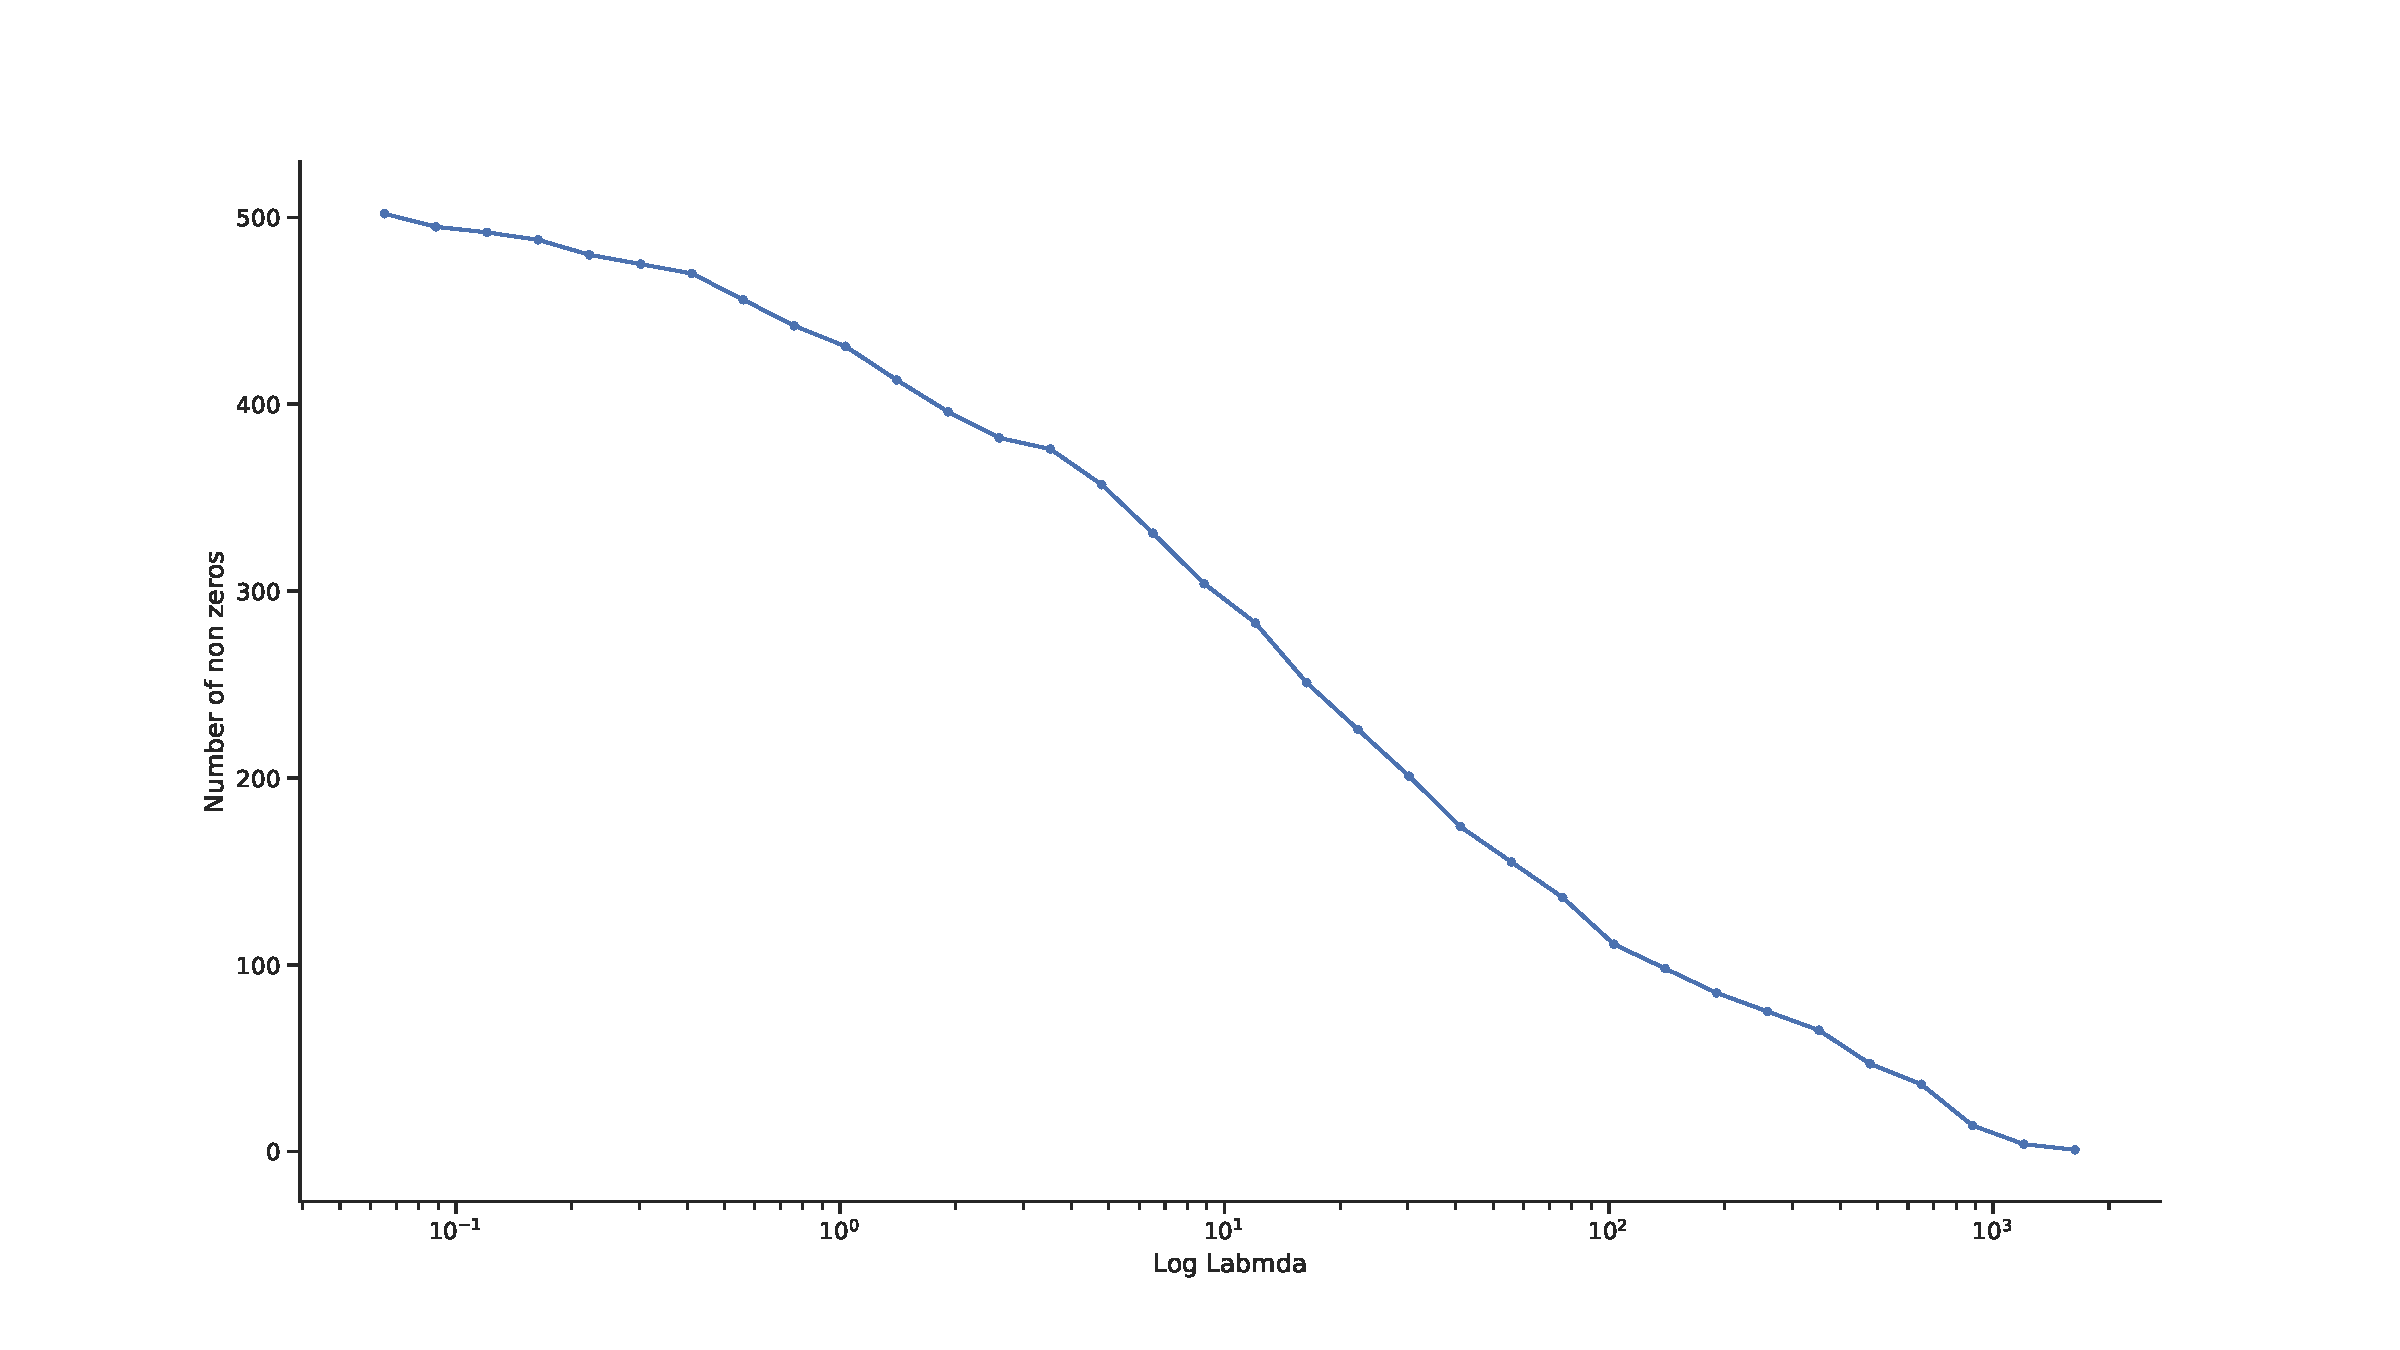
\includegraphics[width=\textwidth]{hw2/P3part1.pdf}
As Lambda increases the number of non zeros goes down. This is because the regularization term starts to dominate the objective function, forcing the norm of w to because small making most of the w terms zero. 

\section*{Problem 3 Part 2}
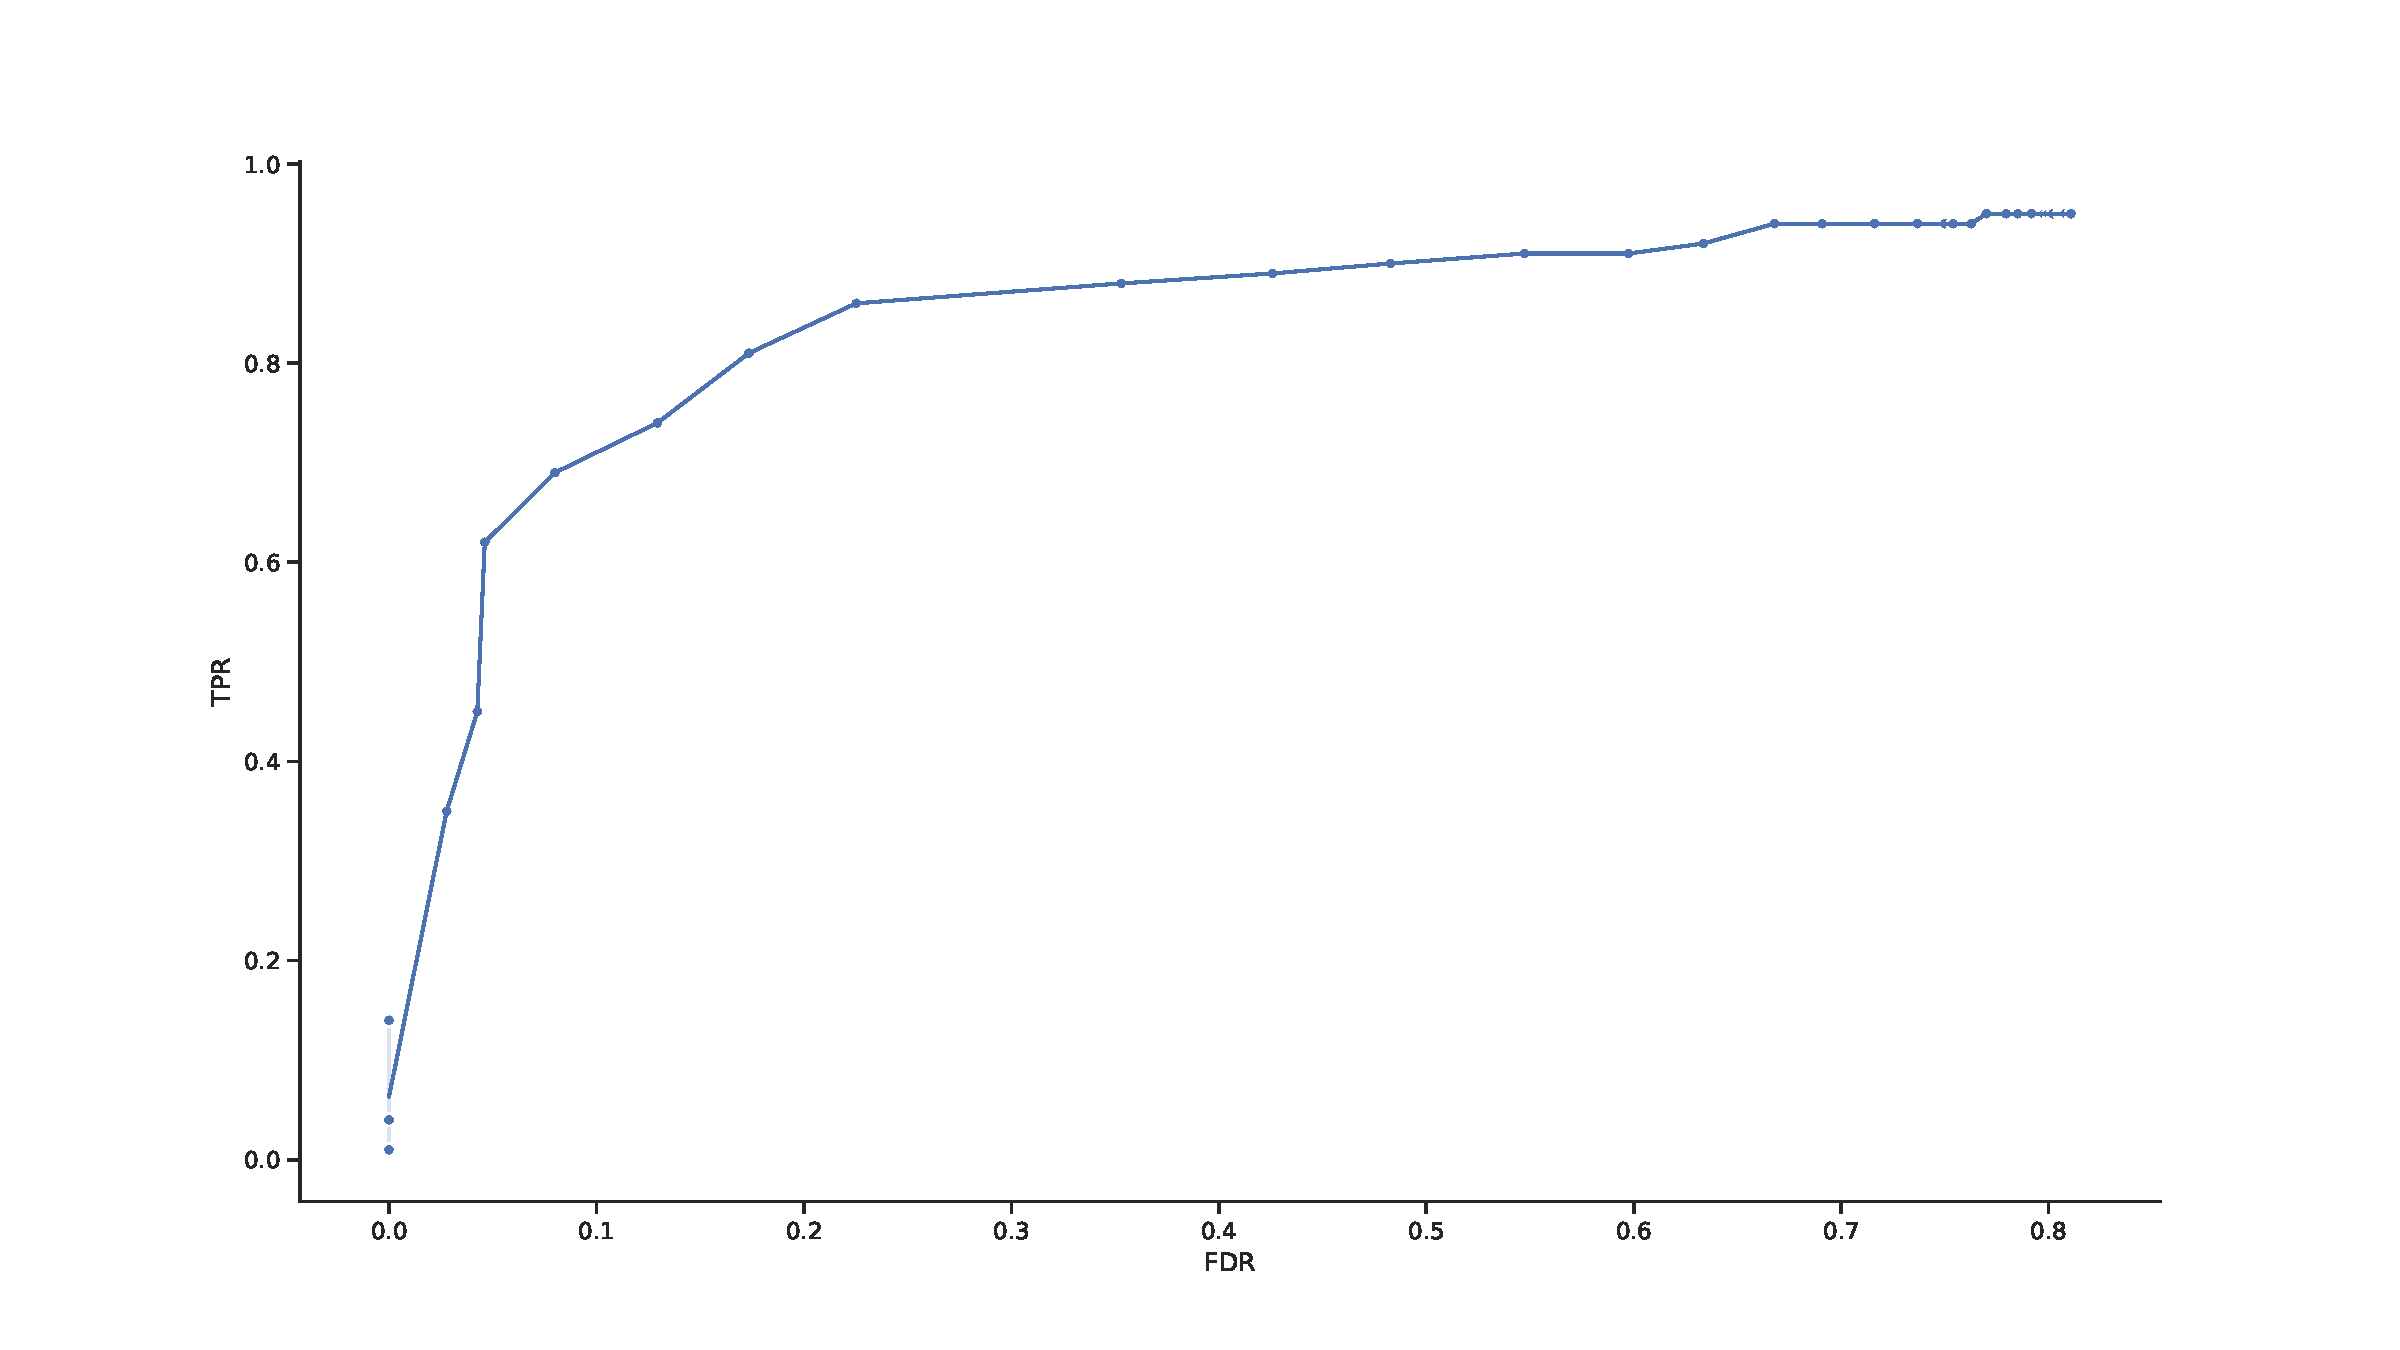
\includegraphics[width=\textwidth]{hw2/P3part2.pdf}
As lambda does down the FDR or number of false positive non zeros goes up. This is because the regularization term is small and not encouraging zero value w terms.  \\

As lambda goes down the number of true positives (TPR) also goes up because we get increased sensitivity because many w terms are non zero. \\

Ideally TPR would increase much more quickly than FDR, and then we would choose the value of lambda that maximizes the trade-off between TPR and FDR for the application. 























\section*{}
4. \grade{5} We'll now put the Lasso to work on some real data from Yelp (an old Kaggle competition, see \url{http://www.kaggle.com/c/yelp-recruiting} for background, but get the data from the class website).

For this competition, the task is to predict the number of useful upvotes a particular review will receive. 
One of the most important requirements for learning great models is creating great features.  
We can use our Lasso solver for this as follows.  First, generate a large amount of features from the data, even if many of them are likely unnecessary.  Afterward, use the Lasso to reduce the number of features to a more reasonable amount. 

Yelp provides a variety of data, such as the review's text, date, and restaurant, 
as well as data pertaining to each business, user, and check-ins.  We have preprocessed this data for you into the following files:

\begin{center}
\begin{tabular}{l l}
\texttt{upvote\_data.csv} & Each row is a review, each column is a real-valued feature ($ n\times d$)  \\
\texttt{upvote\_labels.txt} &  Each row is the number of useful vote counts for that review ($n \times 1$)\\
\texttt{upvote\_features.txt} & Names of each feature for interpreting results ($d\times 1$)
\end{tabular}
\end{center}

To get you started, the Python following code should load the data:

\begin{verbatim}
import numpy as np
# Load a csv of floats:
X = np.genfromtxt("upvote_data.csv", delimiter=",")
# Load a text file of integers:
y = np.loadtxt("upvote_labels.txt", dtype=np.int)
# Load a text file of strings:
featureNames = open("upvote_features.txt").read().splitlines()
\end{verbatim}

Use the first 4000 samples for training, the next 1000 samples for validation, and the remaining samples for testing.
Each sample is a $(x_i,y_i)$ pair. As a pre-processing step, take the square root of each $y_i$ so that $y_i \mapsto \sqrt{y_i}$. This rescaling ameliorates for outliers.
\begin{enumerate}
  \item Solve lasso to predict the number of useful votes a Yelp review will receive.  
  Starting at $\lambda_{max}$, run Lasso on the training set, decreasing $\lambda$ using
  previous solutions as initial conditions to each problem. Stop when you have
  considered enough $\lambda$'s that, based on validation error, you can
  choose a good solution with confidence (for instance, when validation
  error begins increasing by a lot).
  Plot the squared error on the training and validation data versus $\lambda$.
  On a different plot, plot the number of nonzeros in each solution versus $\lambda$.
   (Tip: use \verb|plt.xscale('log')| and \verb|plt.gca().invert_xaxis()|)\\
  \item Find the $\lambda$ that achieves best validation
  performance, and test your model on the remaining set of test data.  What is the train, val, and test error for this choice?
  \item Inspect your solution and take a look at the 10 features with weights largest in magnitude.
  List the names of these features and their weights, and comment on if the weights generally make sense intuitively. As you use a larger $\lambda$ so that fewer features are selected, they may make more sense.
\end{enumerate}  

\subsection{Programming: Binary Logistic Regression}









\section*{Problem 4 Part a}
\includegraphics[width=\textwidth]{hw2/{P4partA.2}.pdf}
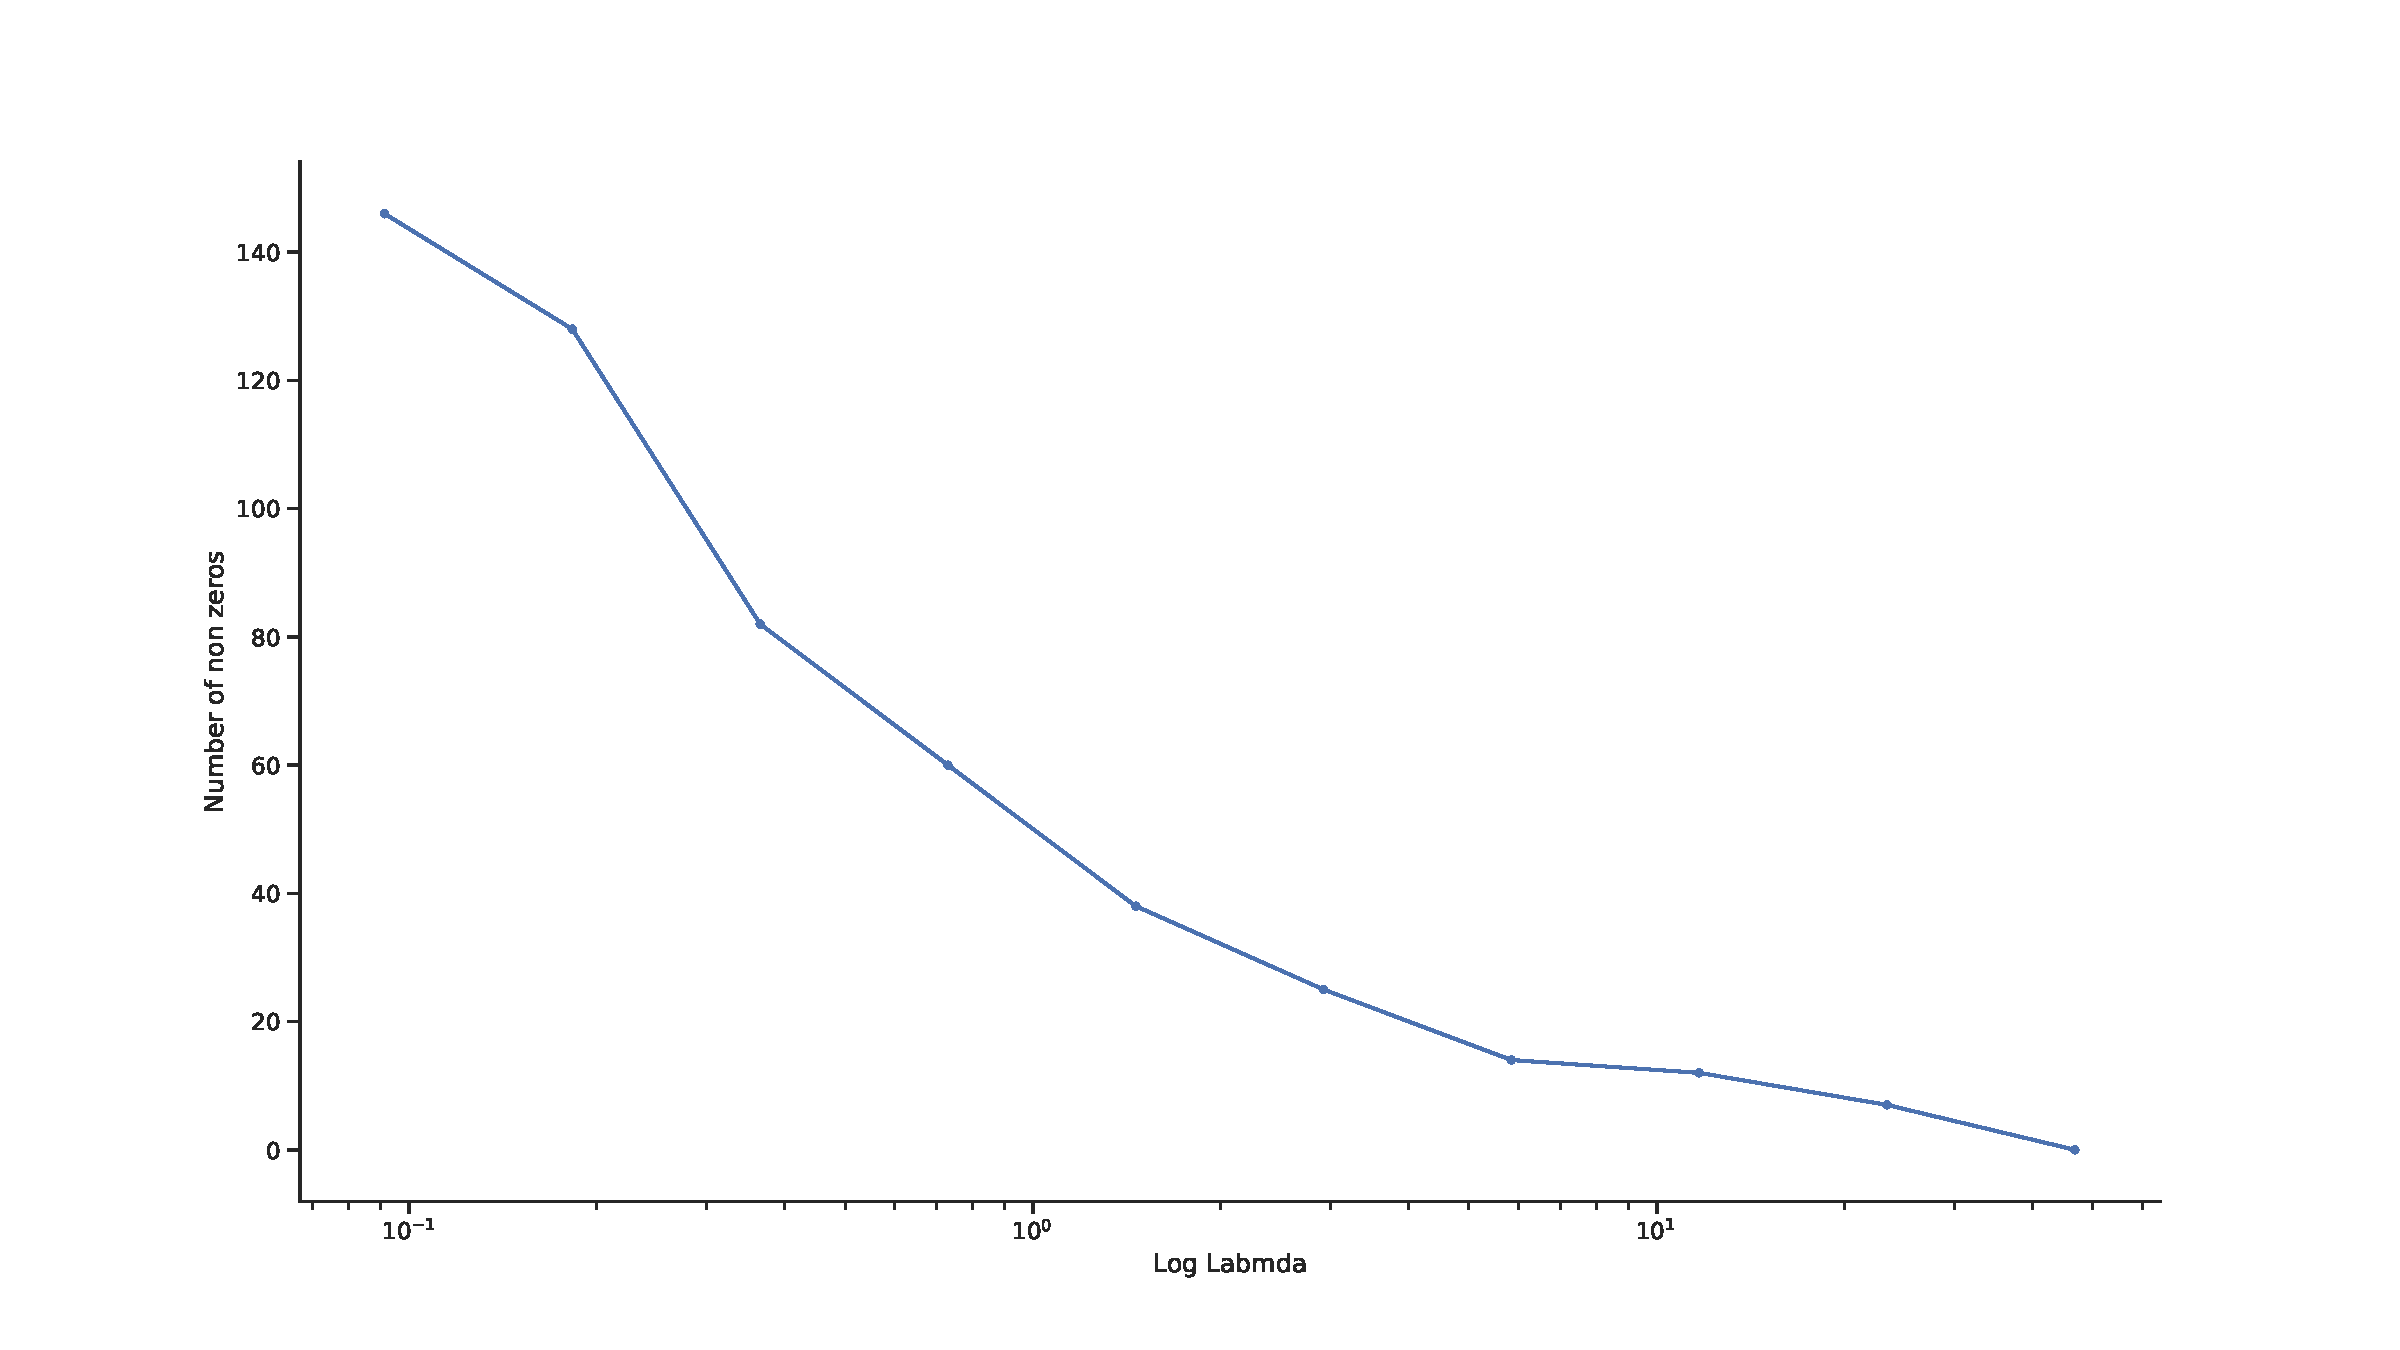
\includegraphics[width=\textwidth]{{hw2/P4partA.1}.pdf}


\section*{Problem 4 Part b}
I found that $\lambda = 0.7309$ optimized my validation MSE.\\
The values I got for train, val, and test were:\\
Train error:0.42780796536013793 \\
Validation error:0.3975071173226106 \\
Test error:0.47285731297083106

\section*{Problem 4 Part c}
Here are all the weights with the features listed after, and a comment on why it is a predictive weight after that. \\
18.5018033432417:sqrt(UserCoolVotes*BusinessNumStars) \\
How positive the review was weighted by the reviewer's reputation. \\ \\
8.77590786132888:log(ReviewNumCharacters*UserUsefulVotes) \\
Effort put into the review weighted by the number of people who found it useful. \\ \\
7.2086619933626945:sqrt(ReviewNumCharacters*UserFunnyVotes) \\
Similar to above. \\ \\
6.954594910044081:log(ReviewNumLineBreaks*UserCoolVotes) \\
Similar to above. \\ \\
4.731374726088002:sqrt(UserFunnyVotes*BusinessNumStars) \\
How positive the review was weighted by the reviewer's reputation. \\ \\
4.534558543784612:sqrt(ReviewNumCharacters*UserCoolVotes) \\
Effort put into the review weighted by the number of people who found it useful. \\ \\
3.906770872396257:log(UserUsefulVotes) \\
Reviewer's reputation. \\ \\
3.017658610300389:log(UserCoolVotes*BusinessIsOpen) \\
How many cool upvotes the reviewer has weighted by how often the buissnes is open. \\ \\
2.132705373968451:sqrt(ReviewNumStars) \\
Reviewer's opinion. \\ \\
2.1251692074021182:log(UserFunnyVotes*BusinessNumReviews) \\
How much the business is reviewed weighted by whether those reviews are good. \\ \\










\section*{Code for problems 3 and 4}

\lstinputlisting[language=python]{hw2/lasso.py}












\section*{}
5. \grade{5} Let us again consider the MNIST dataset, but now just binary classification, specifically, recognizing if a digit is a $2$ or $7$.
Here, let $Y=1$ for all the 7's digits in the dataset, and use $Y=-1$ for $2$.
We will use use regularized logistic regression. 
Given a binary classification dataset $\{(x_i,y_i)\}_{i=1}^n$ for $x_i \in \R^d$ and $y_i \in \{-1,1\}$ we showed in class that the regularized negative log likelihood objective function can be written as
\begin{align*}
J(w,b) = \frac{1}{n} \sum_{i=1}^n \log( 1 + \exp(-y_i (b + x_i^T w))) + \lambda ||w||_2^2
\end{align*} 
Note that the offset term $b$ is not regularized. 
For all experiments, use $\lambda = 10^{-1}$. 
Let $\mu_i(w,b) = \frac{1}{1+ \exp(-y_i (b + x_i^T w))}$. 
\begin{enumerate}
  \item Derive the gradients $\nabla_w J(w,b)$, $\nabla_{b} J(w,b)$ and Hessians $\nabla_w^2 J(w,b)$, $\nabla_{b}^2 J(w,b)$ and give your answers in terms of $\mu_i(w,b)$ (your answers should not contain exponentials).
  \item Implement gradient descent with an initial iterate of all zeros. Try several values of step sizes to find one that appears to make $J(w,b)$ on the training set converge the fastest. Run until you feel you are near to convergence.
  \begin{enumerate}
    \item For both the training set and the test, plot $J(w,b)$ as a function of the iteration number (and show both curves on the same plot).  
    \item For both the training set and the test, classify the points according to the rule $\text{sign}(b + x_i^T w)$ and plot the misclassification error as a function of the iteration number (and show both curves on the same plot). 
  \end{enumerate}
  Note that you are only optimizing on the training set. The $J(w,b)$ and misclassification error plots should be on separate plots.
  \item Repeat (b) using stochastic gradient descent with batch size of 1. Note, the expected gradient with respect to the random selection should be equal to the gradient found it part (a). Take careful note of how to scale the regularizer.
  \item Repeat (b) using stochastic gradient descent with batch size of 100. That is, instead of approximating the gradient with a single example, use 100.
  \item Repeat (b) using Newton's method.  
\end{enumerate}







\section*{Problem 5a Answer}

Taking the first derivatives with respect to w and then b. Note if $u = 1/(1+a)$ then $a=(1-u)/u$
\begin{align*}
\nabla_w J(w,b) &  = \nabla_w \frac{1}{n} \sum_{i=1}^n \log( 1 + \exp(-y_i (b + x_i^T w))) + \lambda ||w||_2^2 \\
    &  = \frac{1}{n} \sum_{i=1}^n \nabla_w \log( 1 + \exp(-y_i (b + x_i^T w))) + \nabla_w \lambda ||w||_2^2 \\
    &  = \frac{1}{n} \sum_{i=1}^n \frac{- y_i x_i \exp(-y_i (b + x_i^T w)) }{ 1 + \exp(-y_i (b + x_i^T w))} + \nabla_w \lambda ||w||_2^2 \\
    &  = \frac{1}{n} \sum_{i=1}^n \frac{- y_i x_i}{ 1 + \exp(-y_i (b + x_i^T w))}   \left( \exp(-y_i (b + x_i^T w))  \right)  + \nabla_w \lambda ||w||_2^2 \\
    &  = \frac{1}{n} \sum_{i=1}^n - x_i y_i   \mu_i(w,b)   \left( (1- \mu_i(w,b))/( \mu_i(w,b))  \right)  + \nabla_w \lambda ||w||_2^2 \\
    &  = \frac{1}{n} \sum_{i=1}^n  -x_i y_i  \left( 1 - \mu_i(w,b) \right)  + 2\lambda w \\
\text{Derivative} & \text{ with respect to b:} \\    
\nabla_b J(w,b) &  = \nabla_b \frac{1}{n} \sum_{i=1}^n \log( 1 + \exp(-y_i (b + x_i^T w))) + \lambda ||w||_2^2 \\
    &  = \frac{1}{n} \sum_{i=1}^n \nabla_b \log( 1 + \exp(-y_i (b + x_i^T w))) + 0 \\
    &  = \frac{1}{n} \sum_{i=1}^n \frac{- y_i \exp(-y_i (b + x_i^T w)) }{ 1 + \exp(-y_i (b + x_i^T w))} \\
    & \text{Using the same steps in the previous derivative we can simplify to: } \\
    &  = \frac{1}{n} \sum_{i=1}^n  -y_i  \left( 1 - \mu_i(w,b) \right)  \\
\end{align*} 



Taking the second derivatives with respect to w and then b. 
\begin{align*}
\nabla_w^2 J(w,b) &  = \nabla_w \frac{1}{n} \sum_{i=1}^n  -x_i^T y_i    \left( 1 - \mu_i(w,b) \right)  + 2\lambda I\\
\nabla_w^2 J(w,b) &  =  \frac{1}{n} \sum_{i=1}^n  x_i^T y_i  \nabla_w \mu_i(w,b)  + 2\lambda I\\
\text{Now calculating } & \nabla_w \mu_i(w,b)\\
\nabla_w \mu_i(w,b) & = \nabla_w \frac{1}{1+ \exp(-y_i (b + x_i^T w))} \\
    & = -1 \frac{ \nabla_w  1+ \exp(-y_i (b + x_i^T w)) }{ (1+ \exp(-y_i (b + x_i^T w)))^2 } \\
    & =  \frac{ x_i^T y_i  \exp(-y_i (b + x_i^T w)) }{ (1+ \exp(-y_i (b + x_i^T w)))^2 } \\
    & =  x_i^T y_i  \exp(-y_i (b + x_i^T w)) * (\mu_i(w,b))^2  \\
    & =  x_i^T y_i   \frac{1-\mu_i(w,b)}{\mu_i(w,b)}* (\mu_i(w,b))^2  \\
    & =  x_i^T y_i  \mu_i(w,b) (1-\mu_i(w,b))  \\
\text{Thus:} & \\
\nabla_w^2 J(w,b) &  =  \frac{1}{n} \sum_{i=1}^n  (y_i x_i)(y_i x_i^T)  \mu_i(w,b) (1-\mu_i(w,b)) + 2\lambda I \\
\end{align*} 

Now with respect to b.
\begin{align*}
\nabla_b^2 J(w,b) &  = \nabla_b \frac{1}{n} \sum_{i=1}^n  - y_i    \left( 1 - \mu_i(w,b) \right)  + 0 \\
    & \text{Using the same steps in the previous derivative we know: } \\
    &  =  \frac{1}{n} \sum_{i=1}^n  y_i^2   \mu_i(w,b) \left( 1 - \mu_i(w,b) \right) 
\end{align*} 


\section*{Problem 5b Answer}
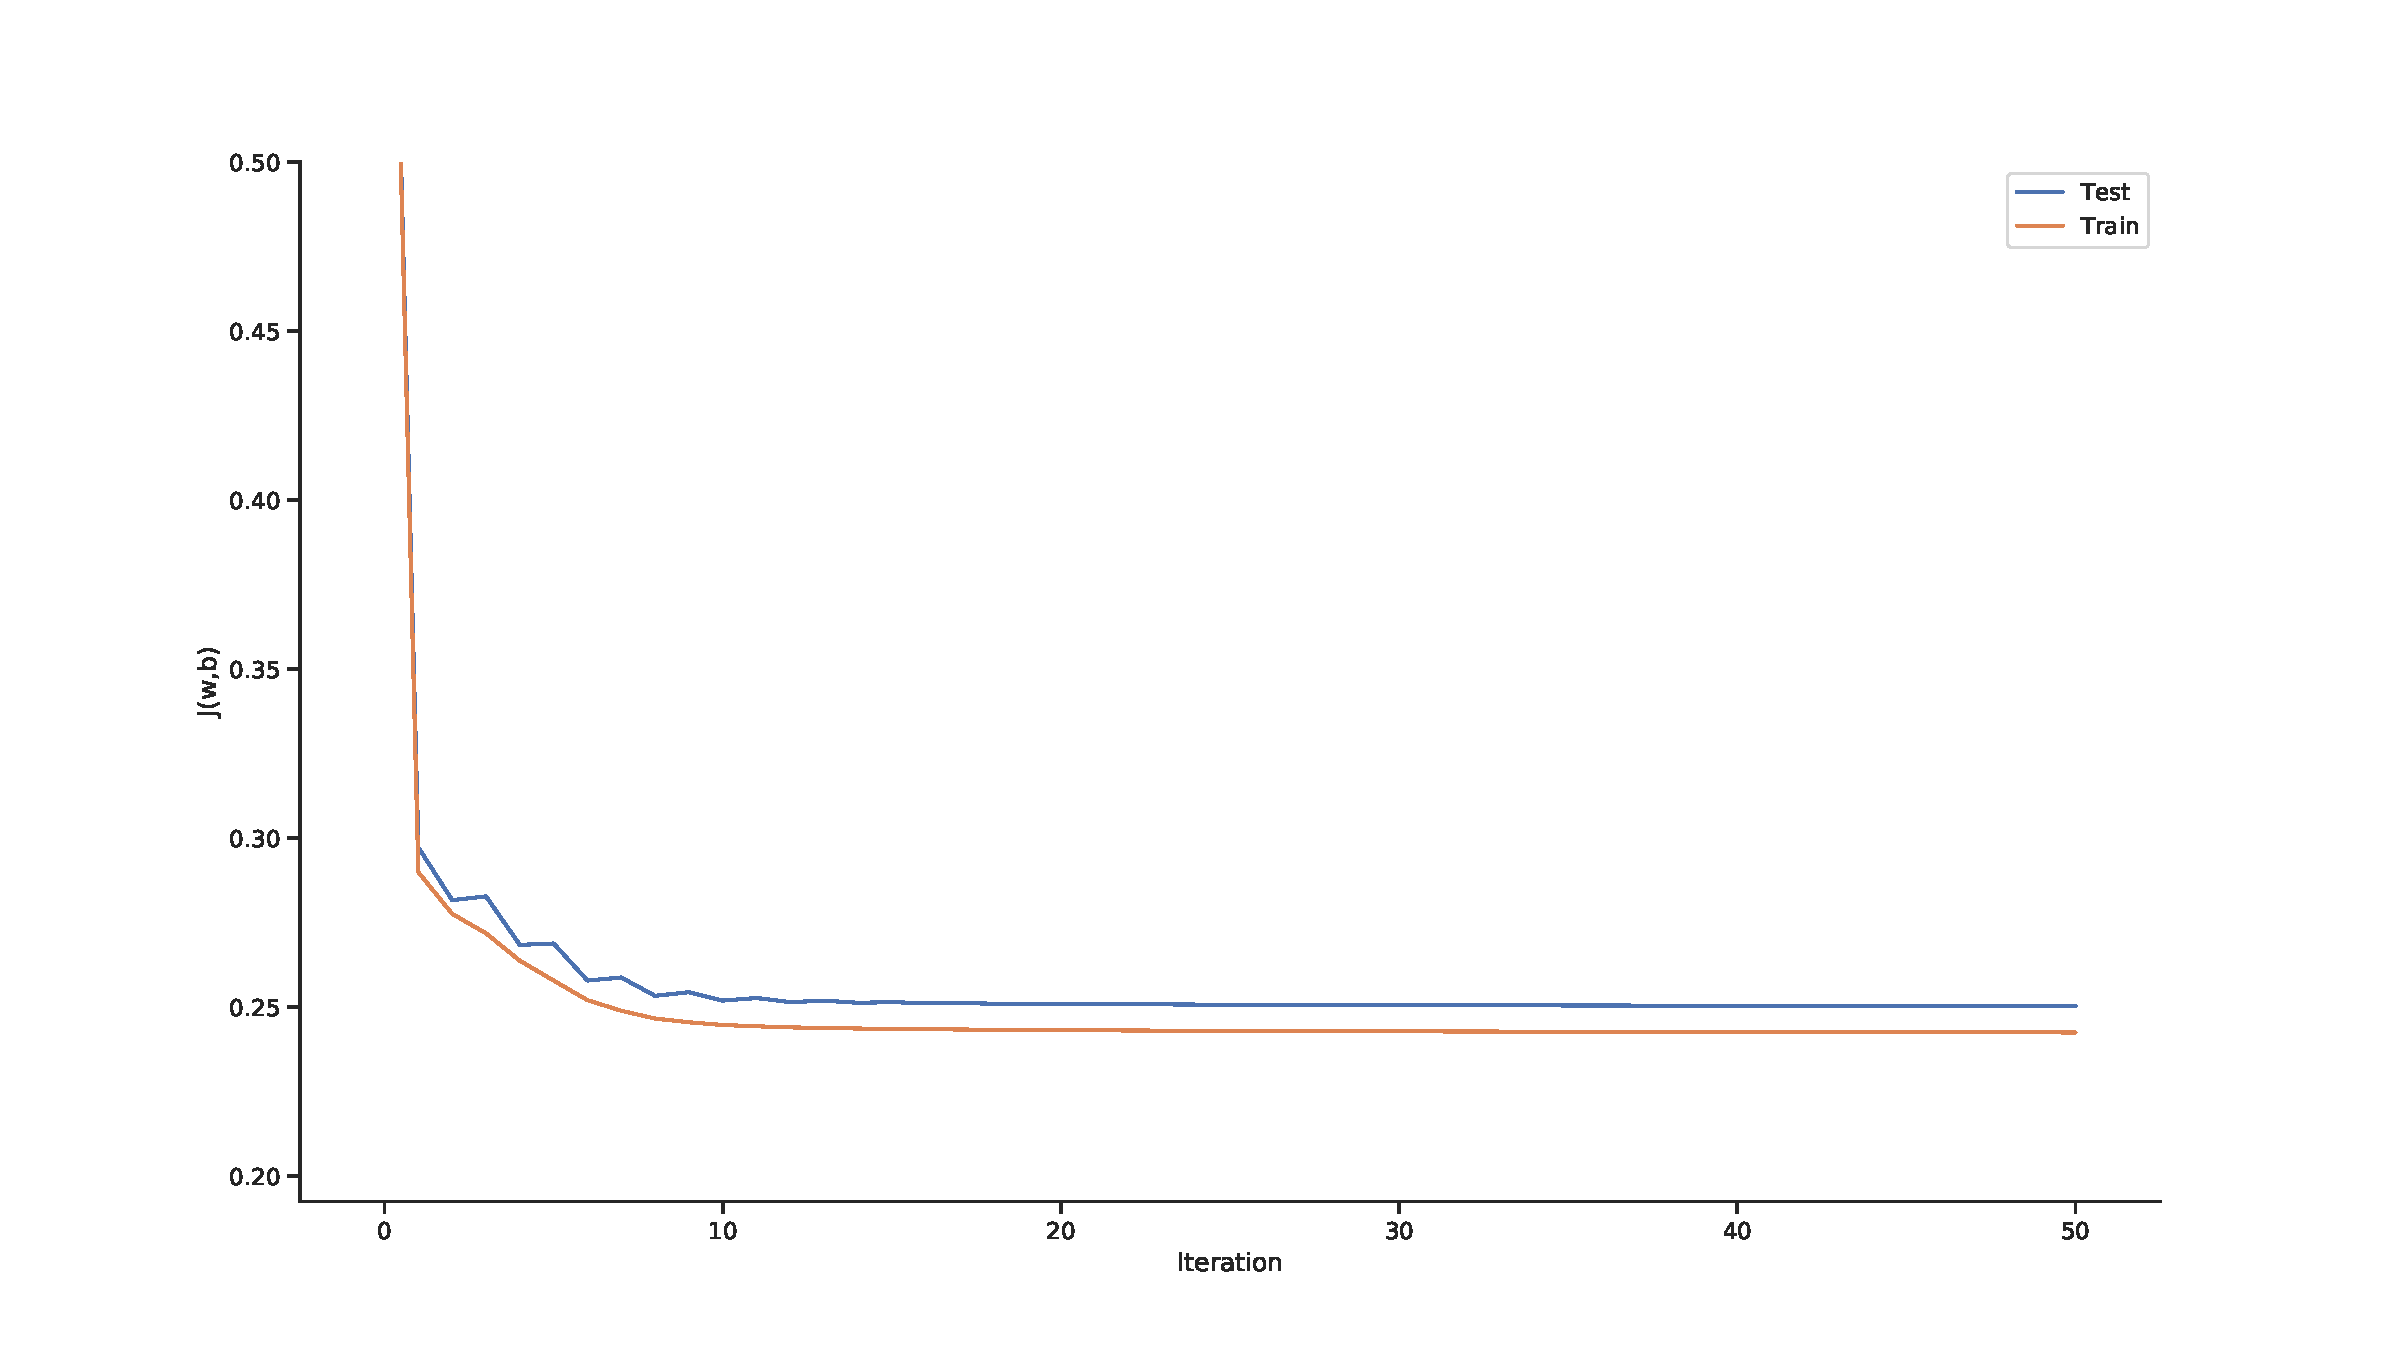
\includegraphics[width=\textwidth]{{hw2/5b.objective}.pdf}
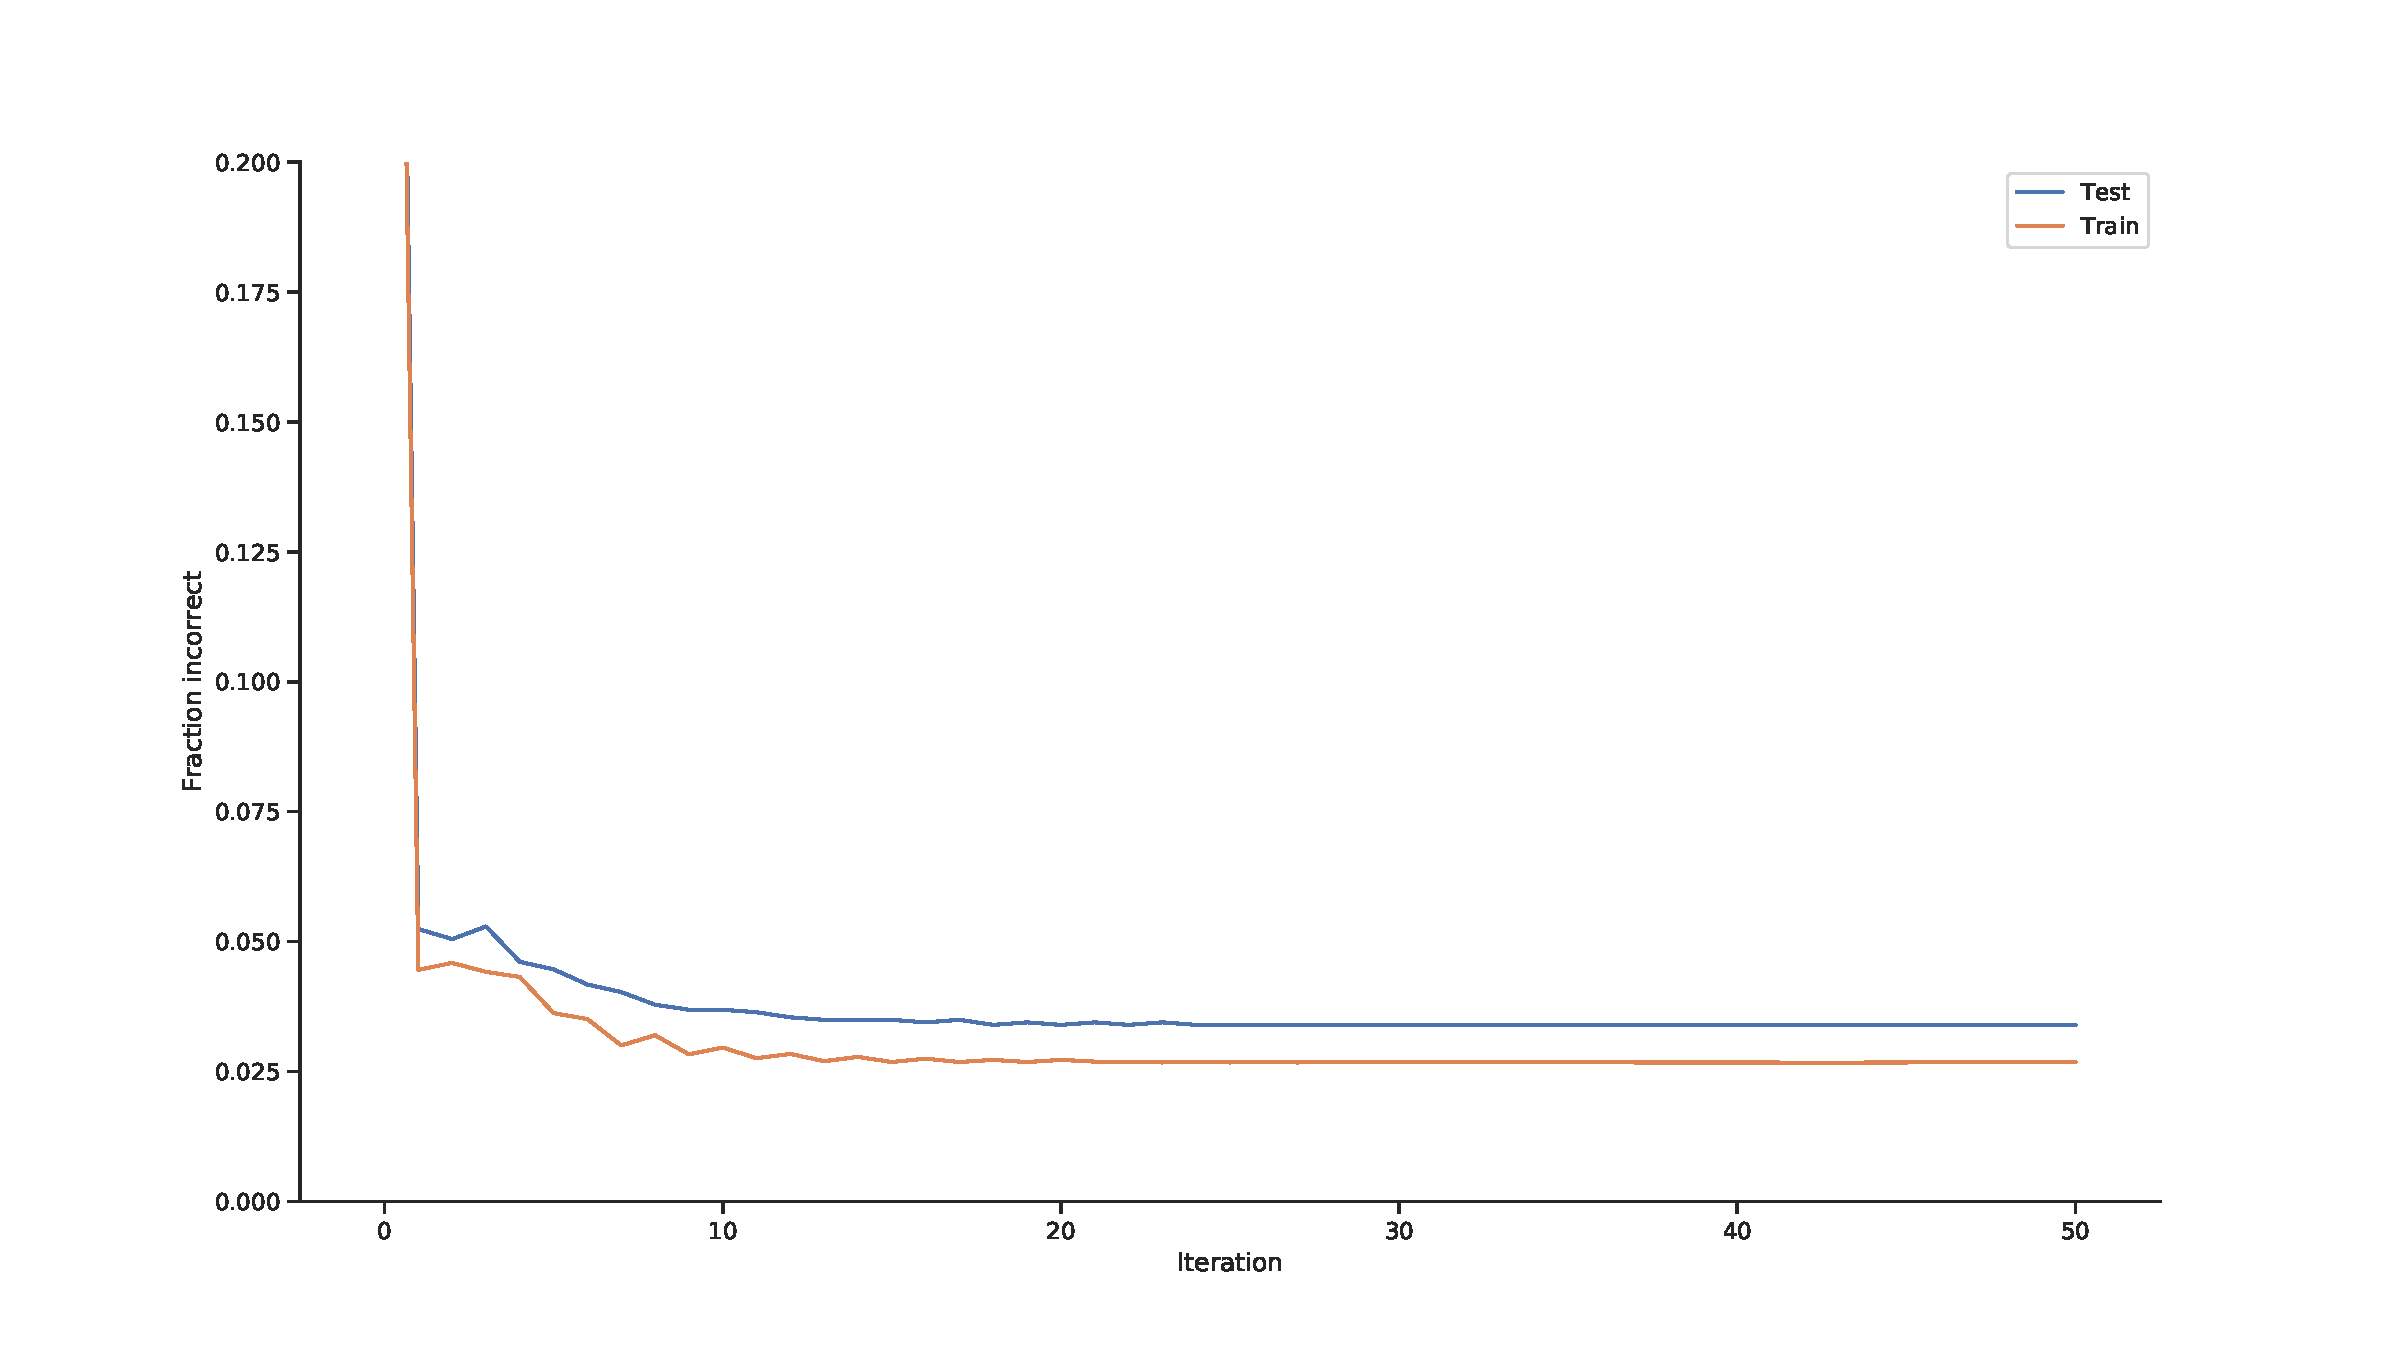
\includegraphics[width=\textwidth]{{hw2/5b.error}.pdf}

\section*{Problem 5c Answer}
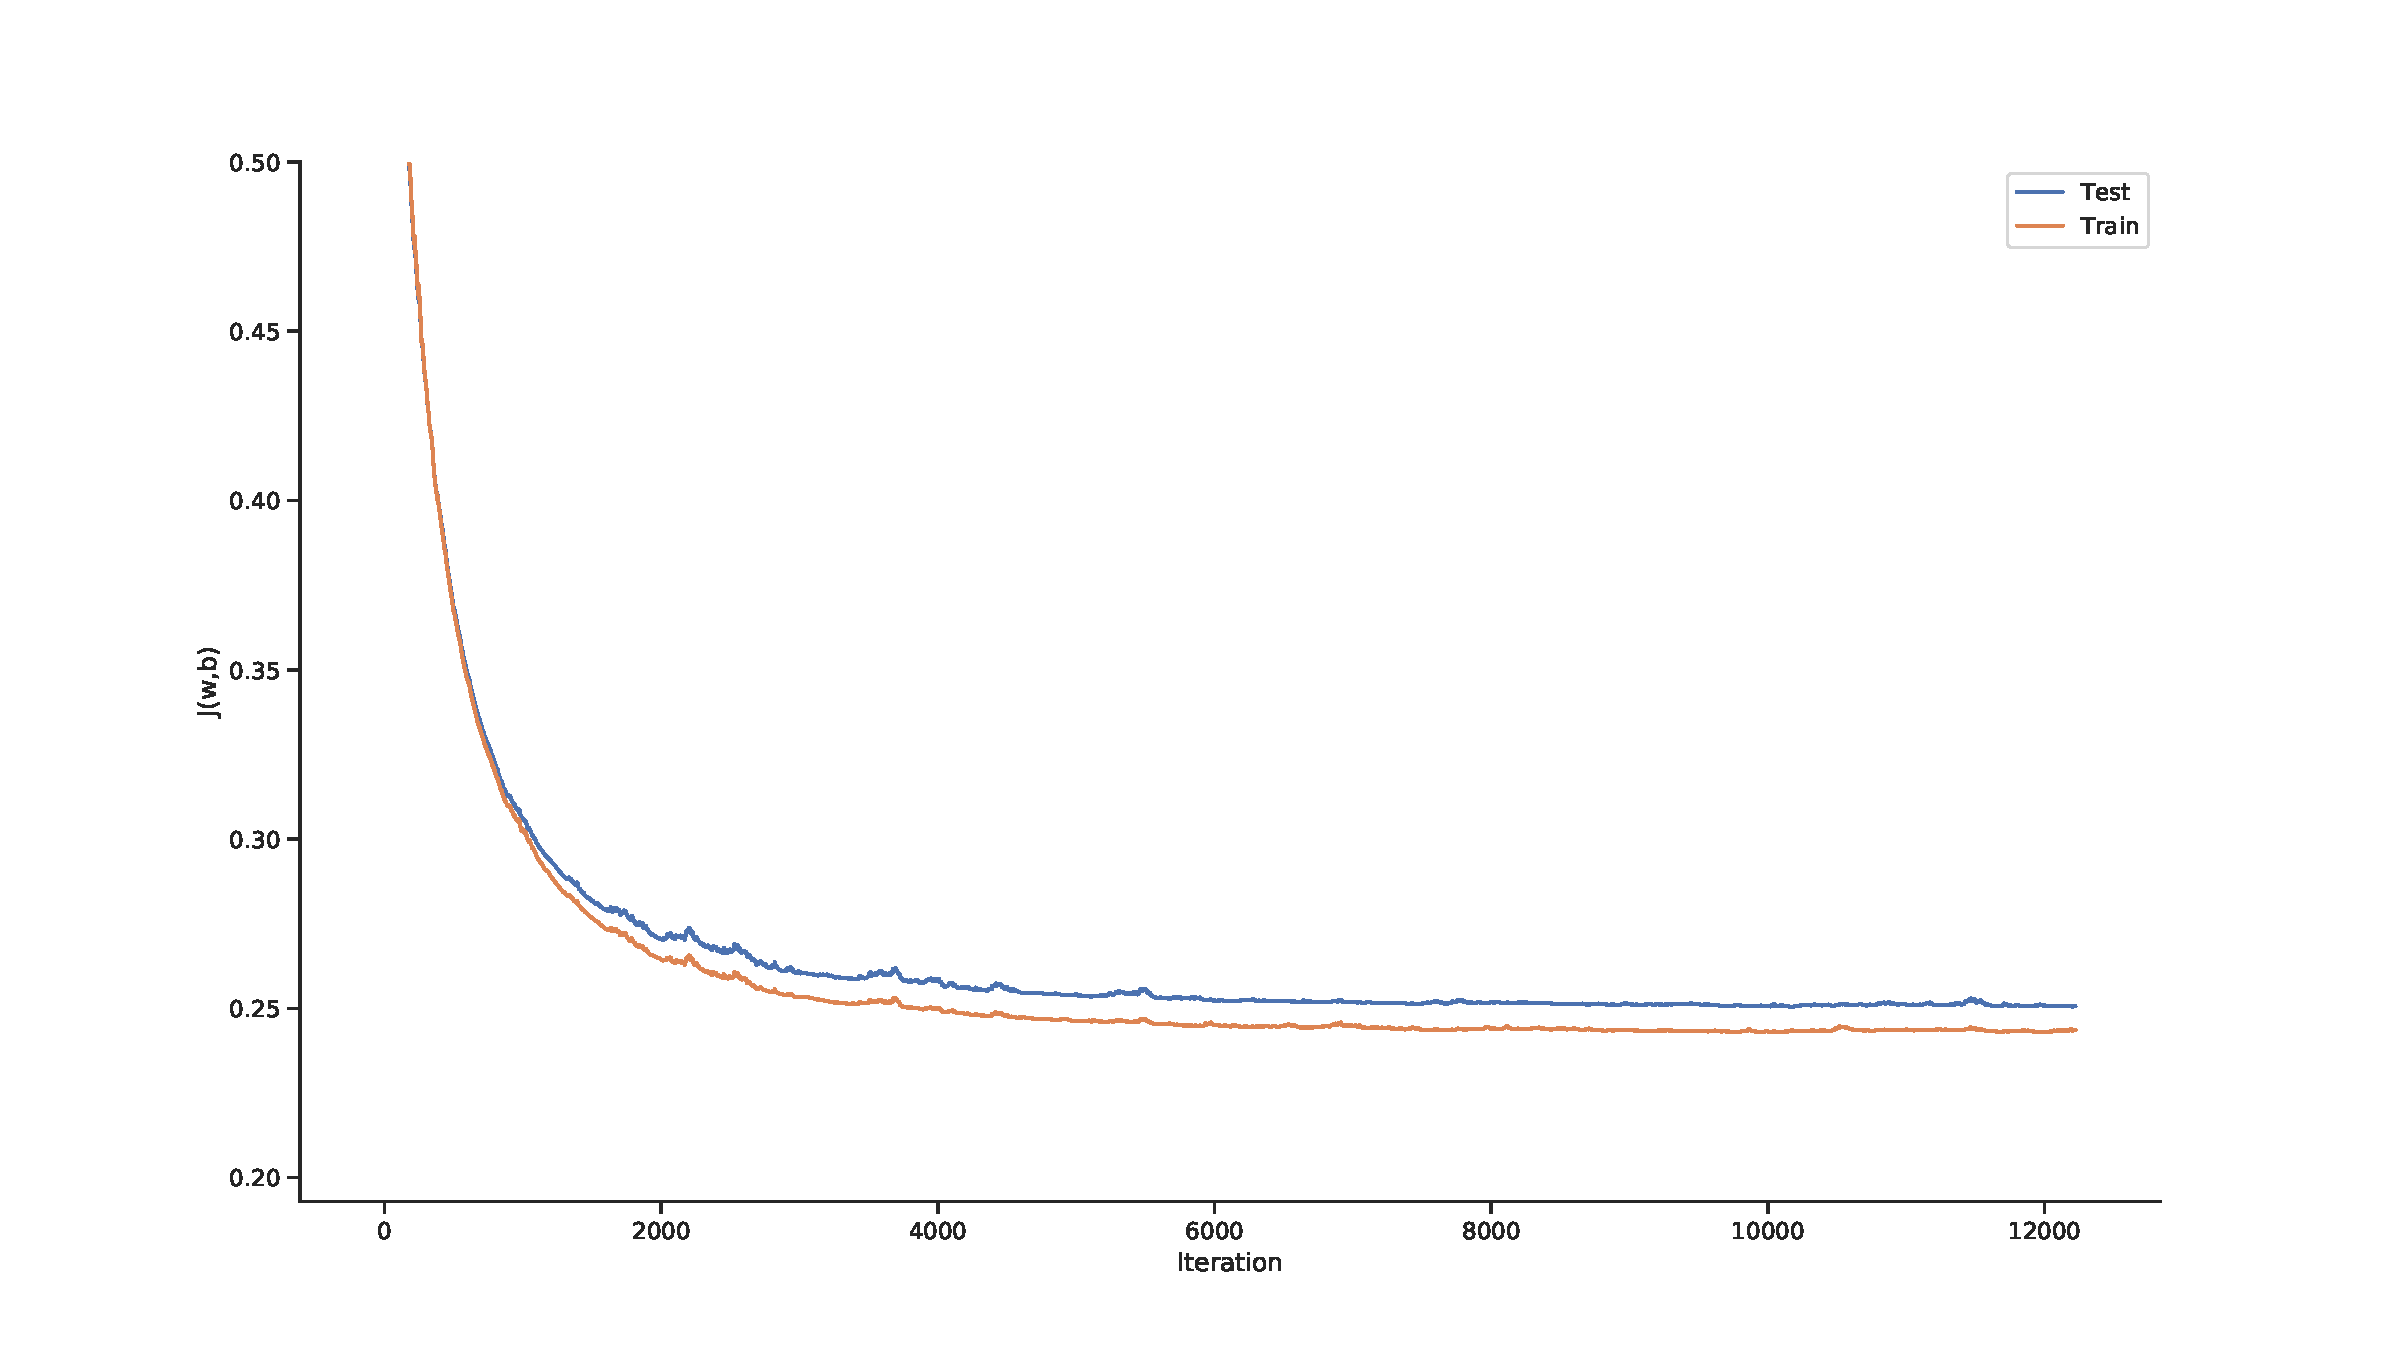
\includegraphics[width=\textwidth]{{hw2/5c.objective}.pdf}
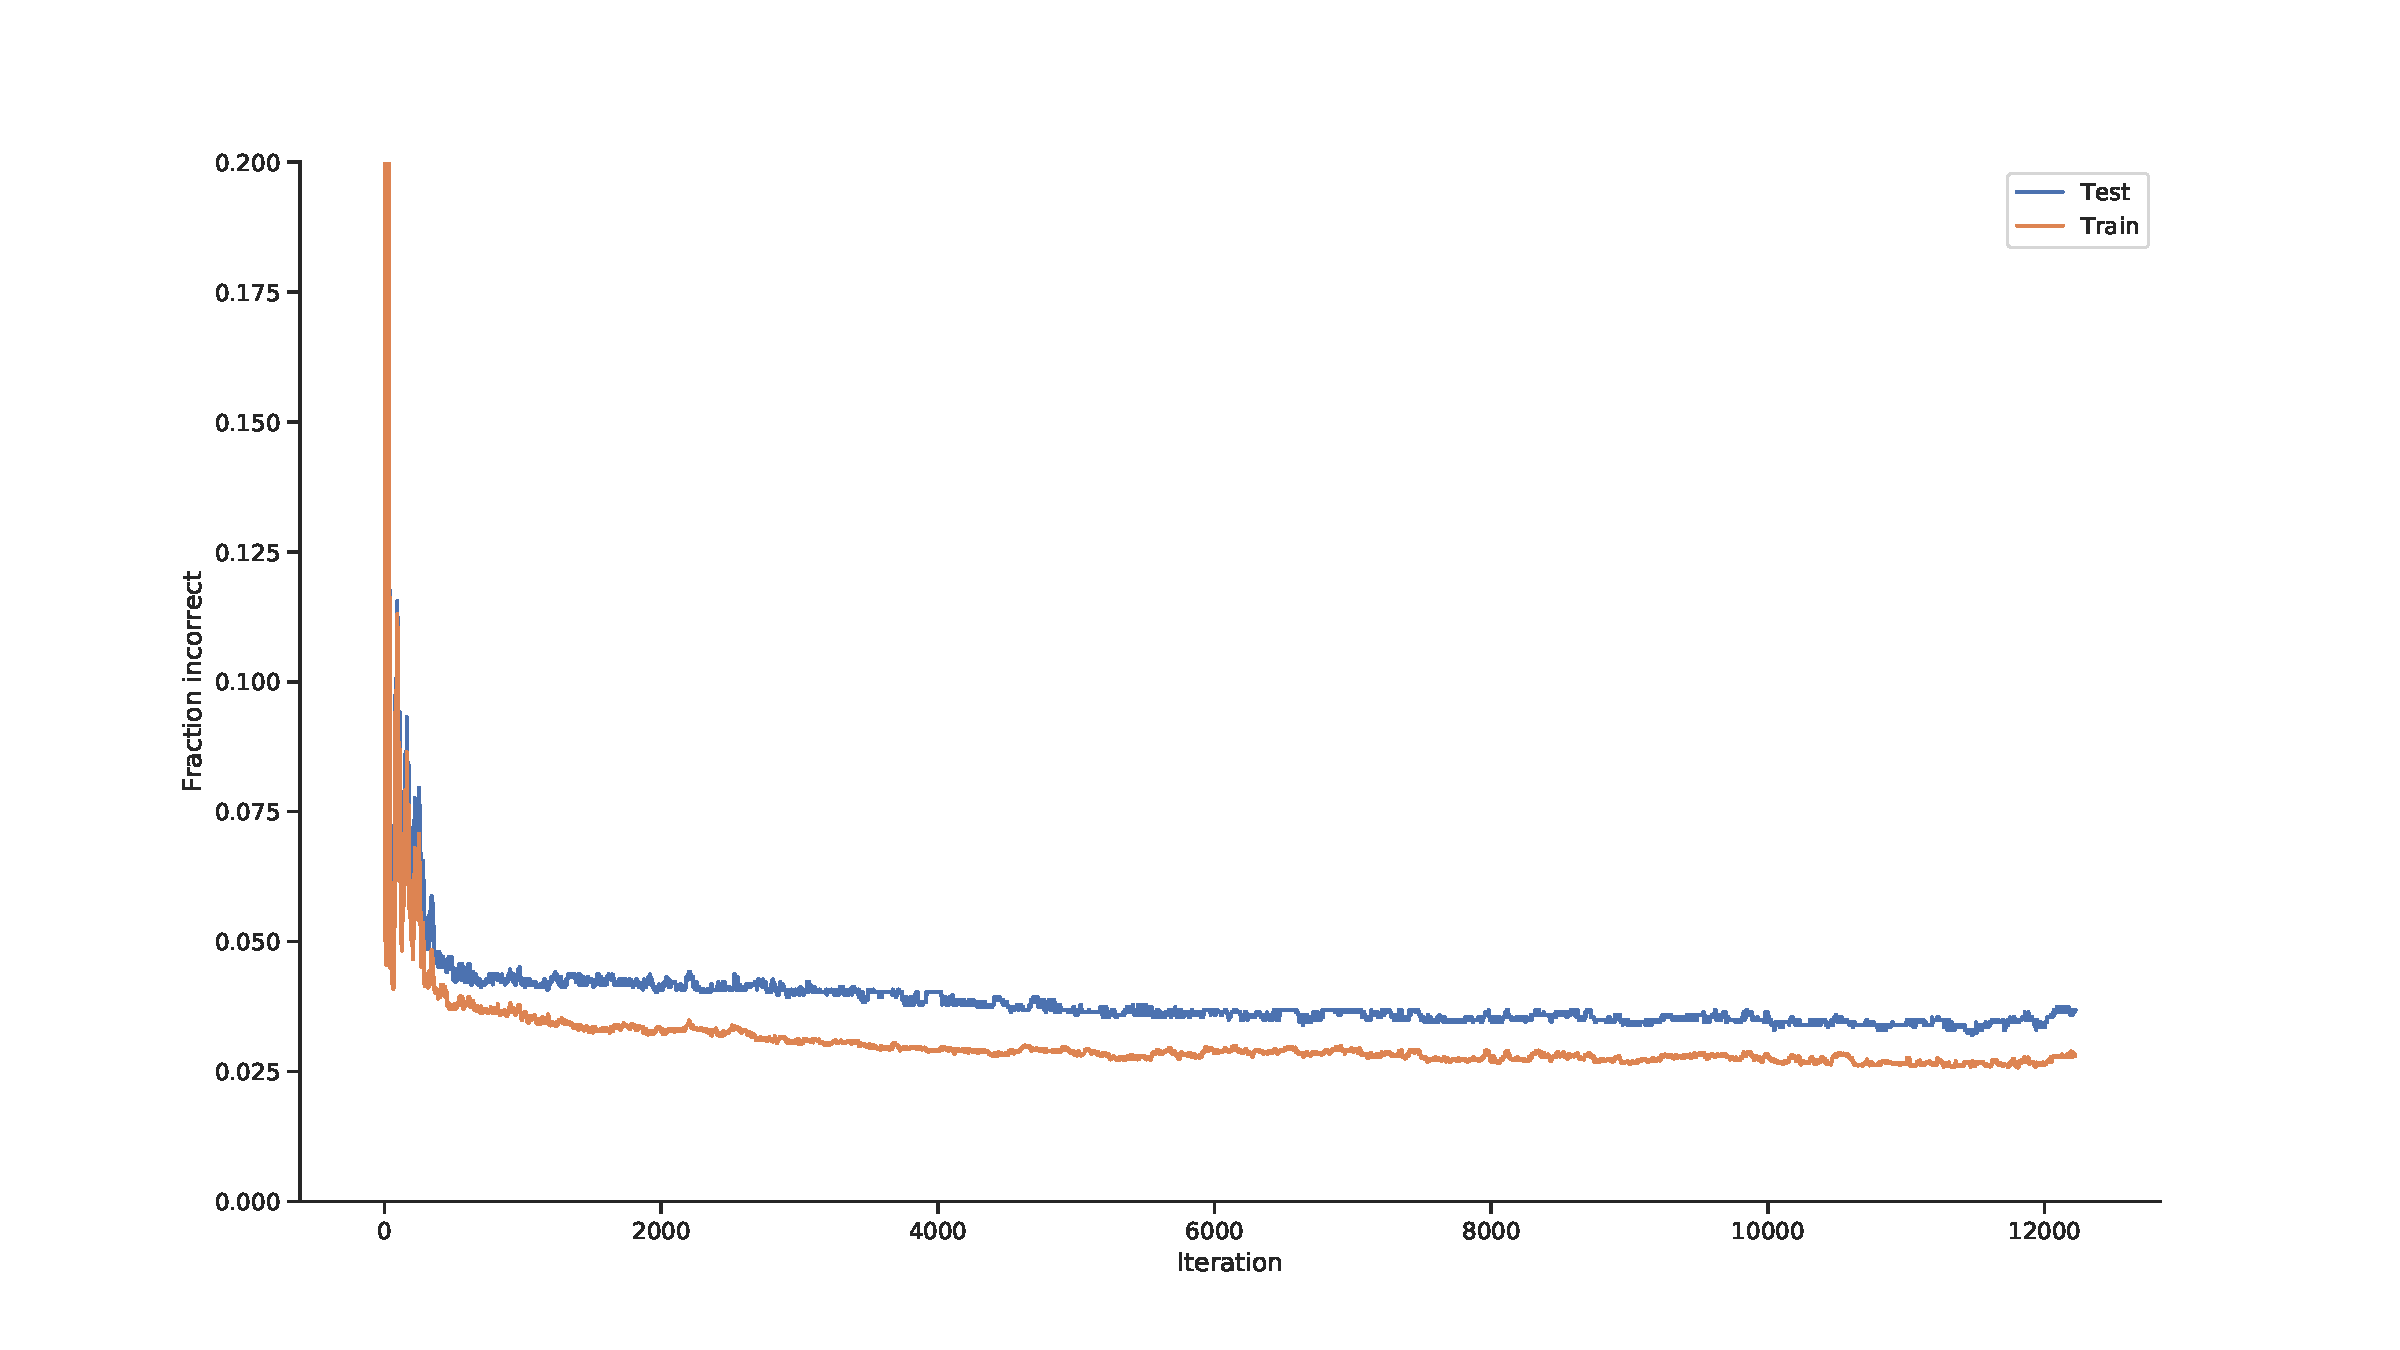
\includegraphics[width=\textwidth]{{hw2/5c.error}.pdf}

\section*{Problem 5d Answer}
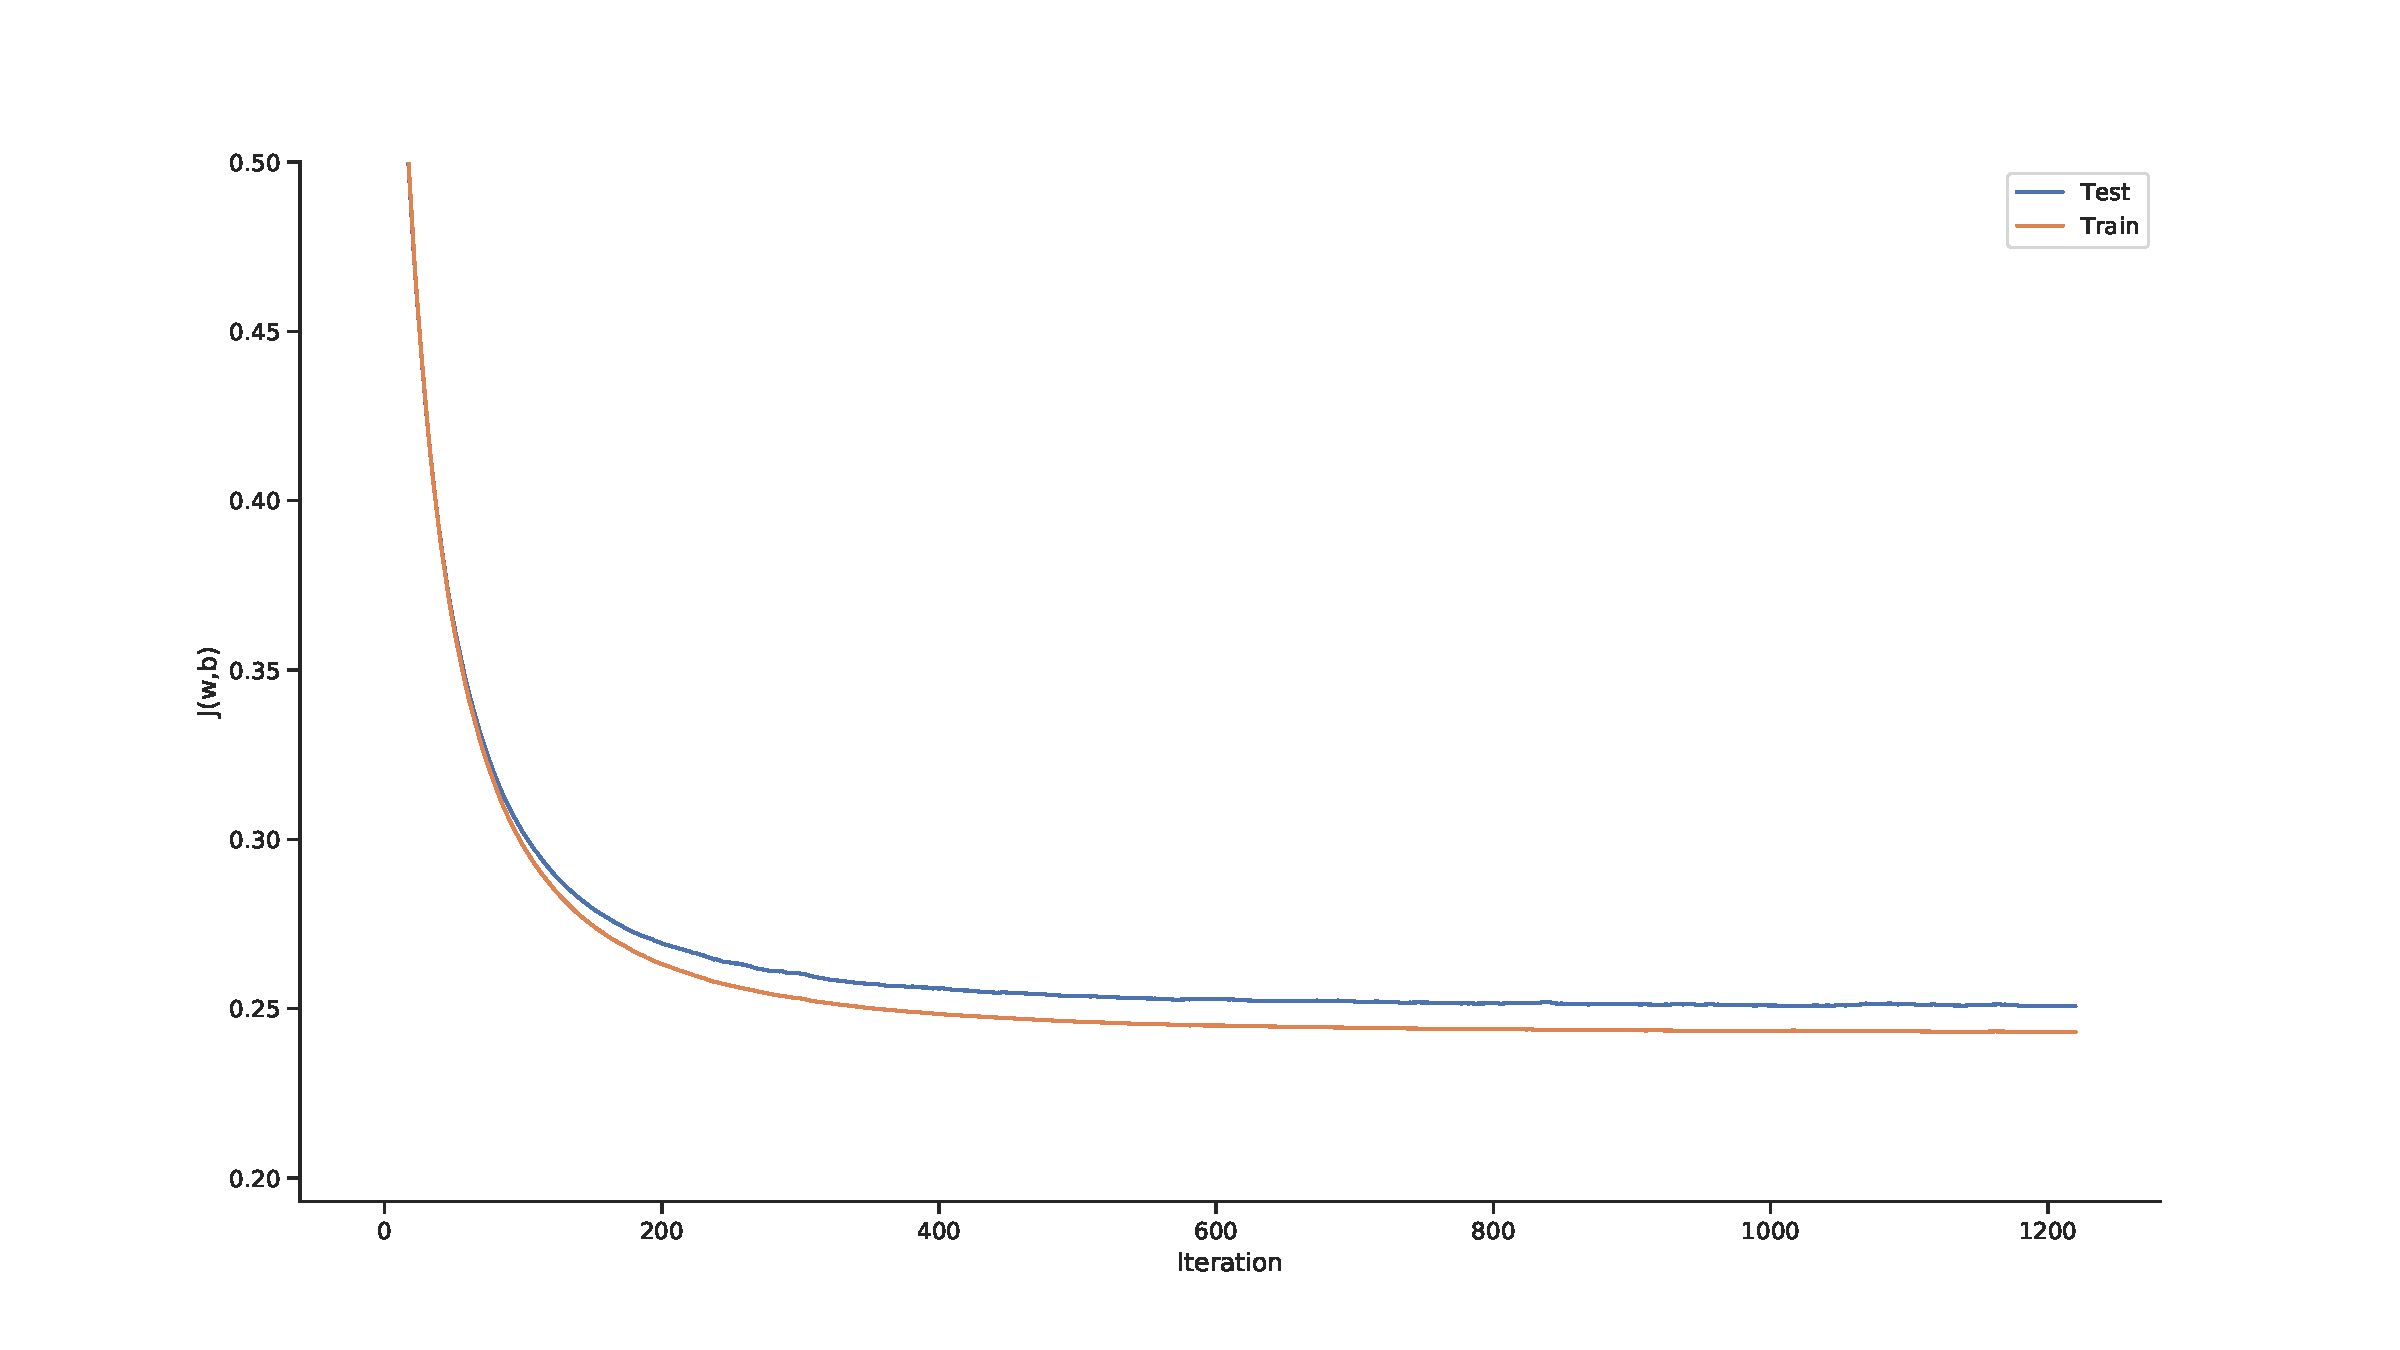
\includegraphics[width=\textwidth]{{hw2/5d.objective}.pdf}
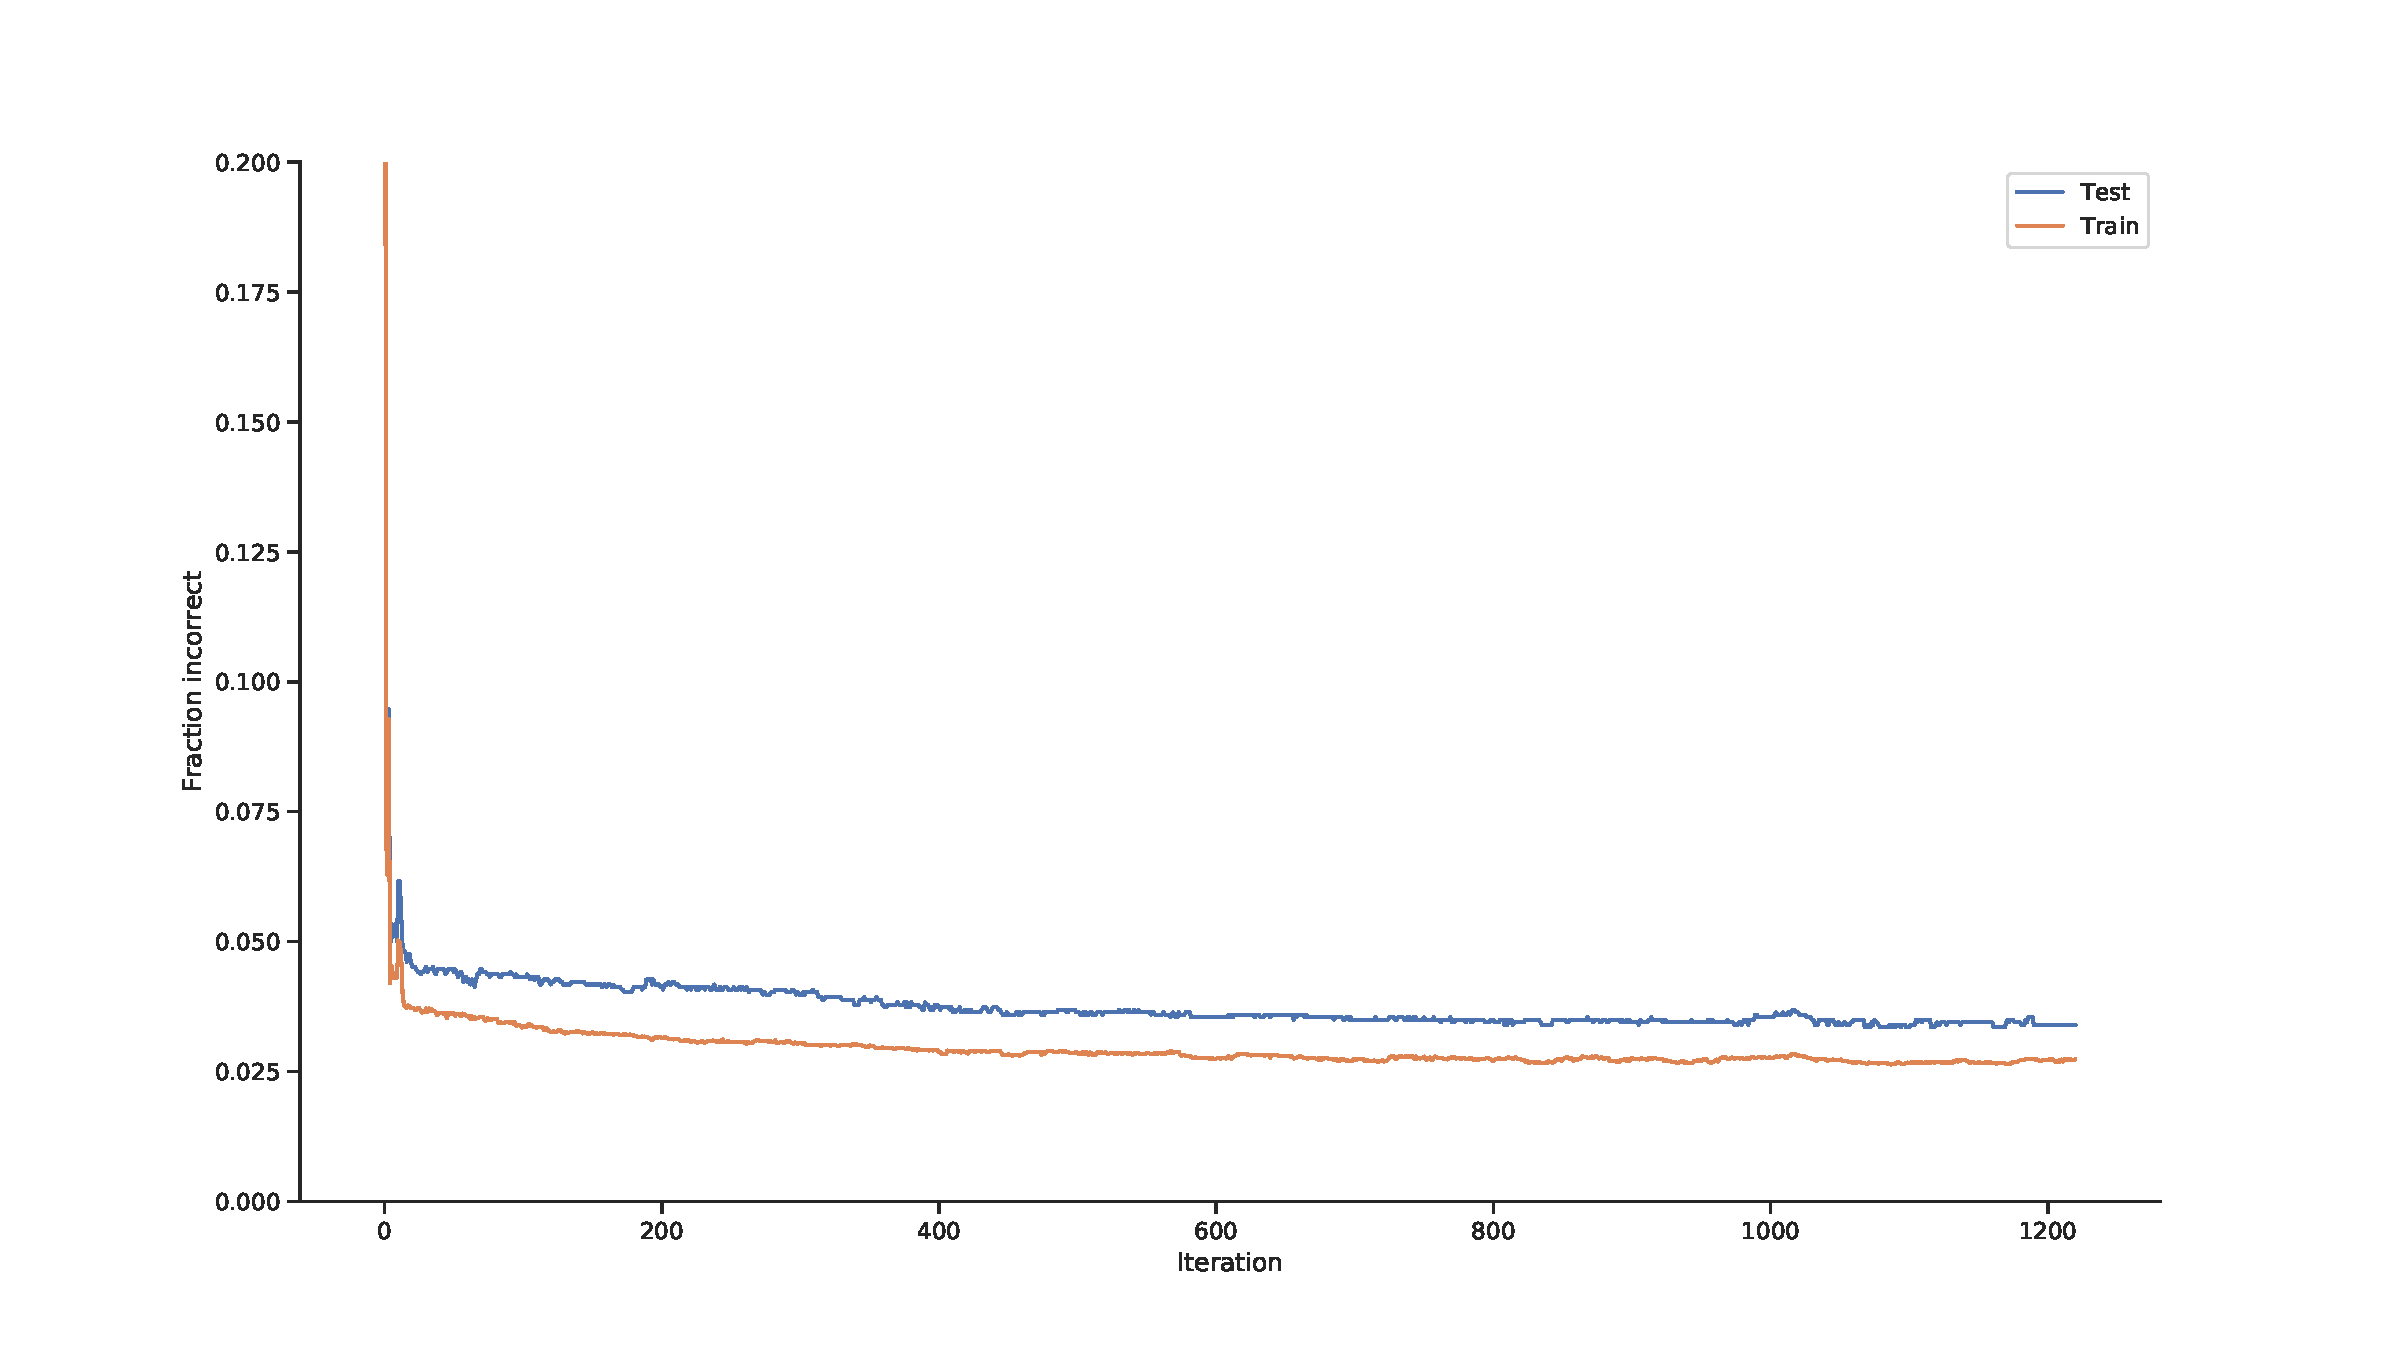
\includegraphics[width=\textwidth]{{hw2/5d.error}.pdf}

\section*{Problem 5e Answer}
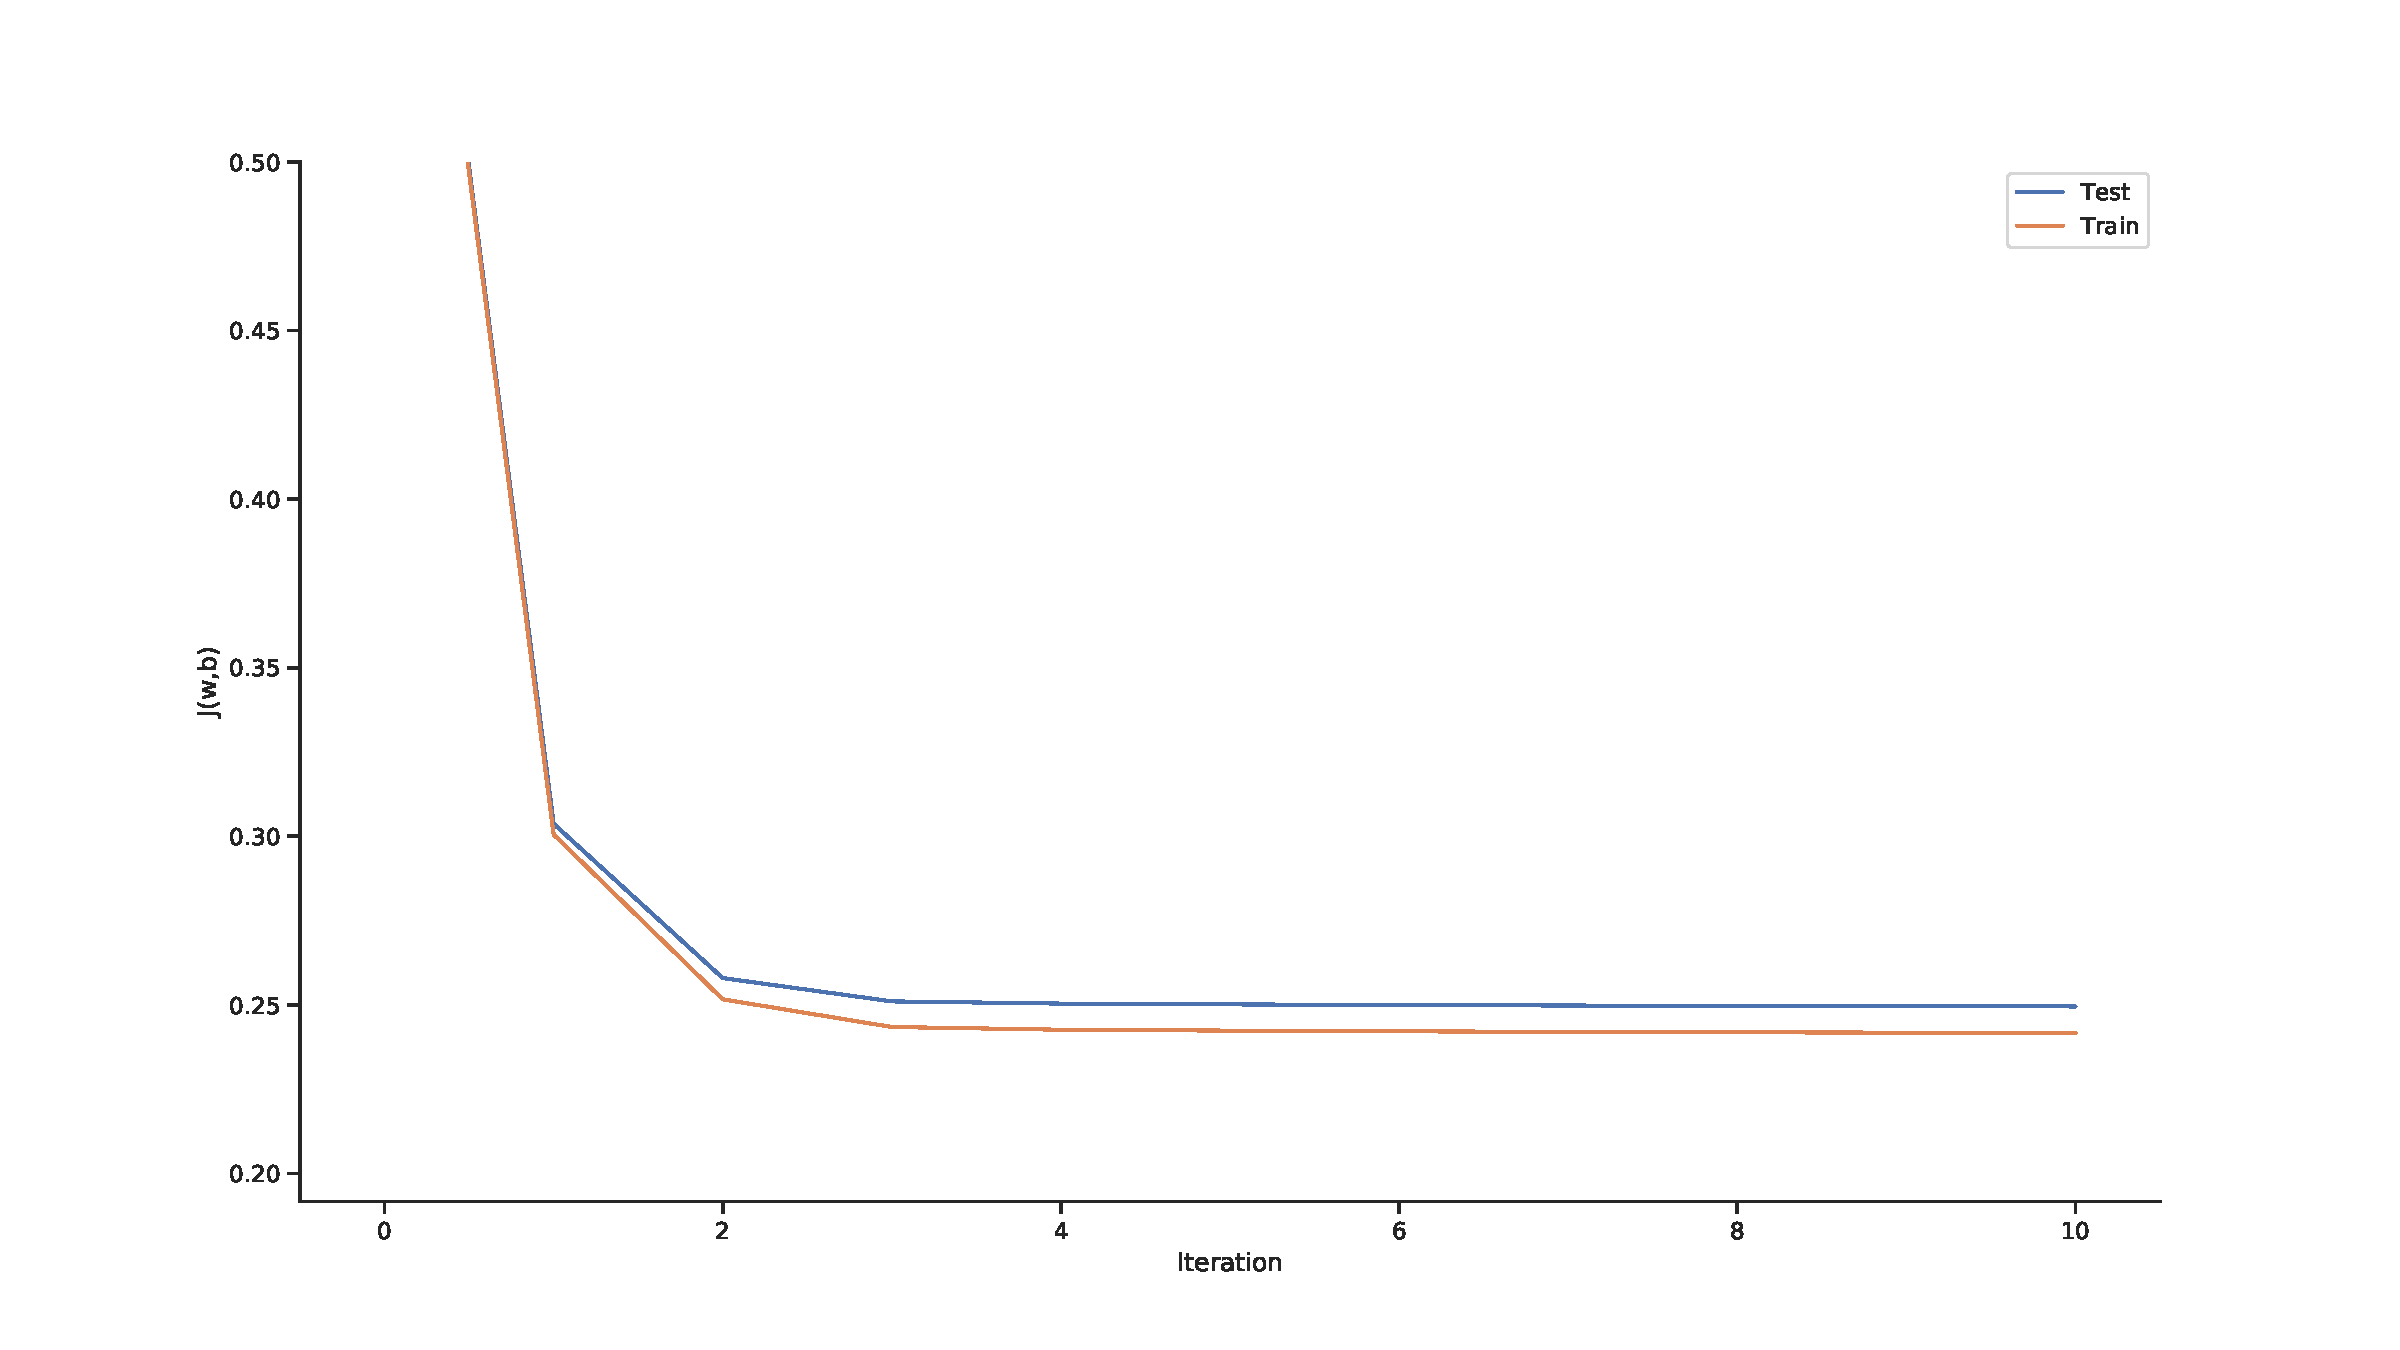
\includegraphics[width=\textwidth]{{hw2/5e.objective}.pdf}
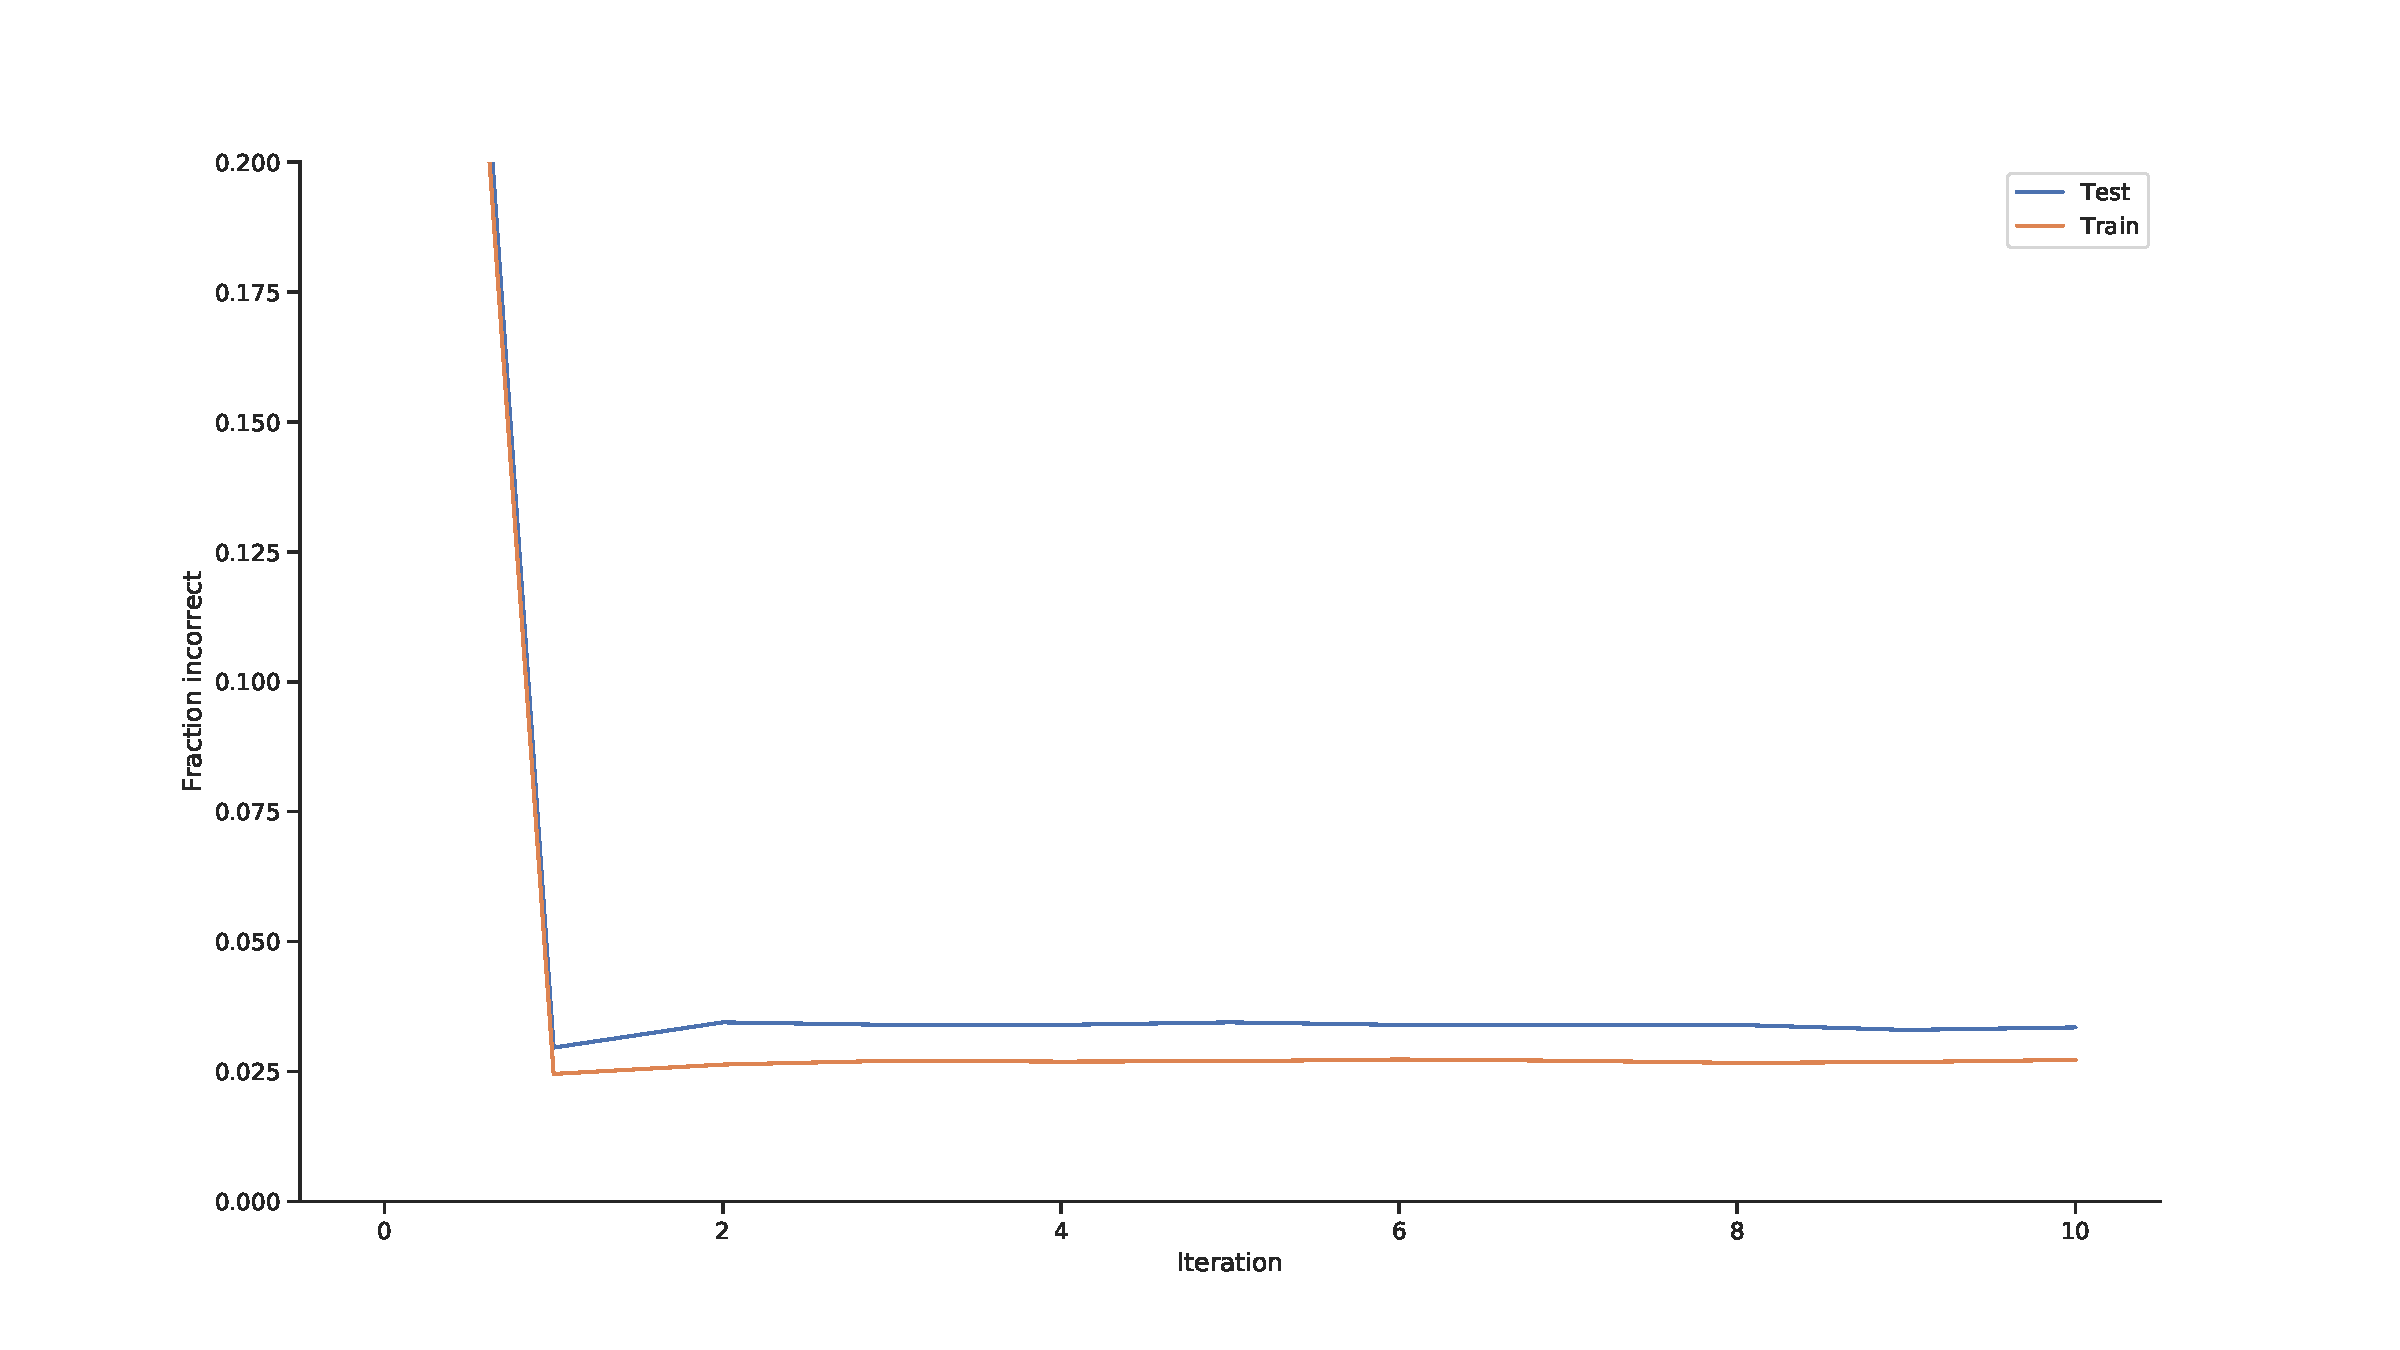
\includegraphics[width=\textwidth]{{hw2/5e.error}.pdf}



\section*{Problem 5 code}
\lstinputlisting[language=python]{hw2/logistic.py}



\end{document}
